%Document vide aux normes de l'École nationale des Chartes
%Dernières modifications E. Rouquette (12/2023)

%%%%%%%%%%%%%%%%%%%%%% PRÉAMBULE


%%%%%%%%%%%%%% partie obligatoire du préambule
\documentclass[a4paper,12pt,twoside]{book}
\usepackage{fontspec}
\usepackage{xunicode}
\usepackage[french]{babel}%on peut préciser d'autres langues.
\usepackage{float}%pour le positionnement des images


%%%%%%%%%%%%%%%%%%%%%%%%%%%%%%%%% PACKAGES UTILISÉS

\usepackage{csquotes} % les guillemets français
\usepackage{lettrine} %faire une lettrine (pas obligatoire)

\usepackage[style=enc,sorting=nyt,maxbibnames=10]{biblatex}%charger le style de l'EnC (téléchargeable ici https://ctan.org/pkg/biblatex-enc)
\addbibresource{BibliographieMemoire.bib} %le fichier bibliograhique. Exemple de chemin à partir du dossier où se trouve le document maître:Exemple ./dossierA/fichier.bib
\defbibheading{Histoire de la BIS et du livre}{\subsection*{Histoire de la BIS et du livre}} 
\defbibheading{OCR et HTR}{\subsection*{OCR et HTR}}  

\nocite{*}


%%%Faire un ou plusieurs index

%\usepackage{imakeidx} %pour faire un ou plusieurs index
%\makeindex %commande pour générer l'index


%RAJOUTEZ ICI VOS PACKAGES




%%%%%%%%%%%%%%%%%%%%%%%%%%%%%%%%% CONFIGURATION DE MISE EN PAGE

%%%%%% Les compteurs (sections, subsections, etc)


%%%%%% Les compteurs (sections, subsections, etc)
\renewcommand{\thesection}{\Roman{section}.}%On ne fait apparaître que le numéro de la section
\renewcommand{\thesubsection}{\arabic{subsection}.}%subsection en chiffres arabes
\renewcommand{\thesubsubsection}{\alph{subsubsection}.}%subsubsection en lettres minuscules
%Si l'on veut faire apparaître les subsubsection dans le table des matières (à commenter sinon)
\setcounter{tocdepth}{3}
\setcounter{secnumdepth}{3}  % La subsubsection (profondeur=3 dans la table des matières) apparait numérotée dans la TdM



%%%%%  Configurer le document selon les normes de l'école

\usepackage[margin=2.5cm]{geometry} %marges
\usepackage{setspace} % espacement qui permet ensuite de définir un interligne
\onehalfspacing % interligne de 1.5
\setlength\parindent{1cm} % indentation des paragraphes à 1 cm

%%%%% Mise en forme des headers (haut de page)

\usepackage{fancyhdr} %package utilisé pour modifier les headers
\pagestyle{fancy} %utiliser ses propres choix de mise en page et non ceux par défaut du package

\setlength\headheight{16pt}%la hauteur des headers
\renewcommand{\sectionmark}[1]{\markright{\small\textit{\thesection~\  #1}}}%Faire apparaître dans les headers les sections en  petit et en italiques
\renewcommand{\sectionmark}[1]{}%Commenter la lign précédetne et mettre celle-ci pour ne pas avoir le titre des sections dans le header
\renewcommand{\chaptermark}[1]{\markboth{\small\chaptername~\thechapter~--\ \textit{#1}}{}}%idem pour les chapitres
%\renewcommand{\chaptermark}[1]{}%Commenter la ligne précédente et mettre celle-ci pour ne pas avoir le titre des chapitres  dans le header



%indiquer des règles d'hyphénation pour des mots précis si besoin
%\begin{hyphenrules}{french}
%	\hyphenation{}
%\end{hyphenrules}


%%%%%%% Package hyperref
% A mettre après les autres appels de packages car redéfinit certaines commandes).

\usepackage[colorlinks=false, breaklinks=true, pdfusetitle, pdfsubject ={Mémoire HN}, pdfkeywords={les mots-clés}]{hyperref} %
\usepackage[numbered]{bookmark}%va avec hyperref; marche mieux pour les signets. l'option numbered: les signets dans le pdf sont numérotés

% Compléter pdfsubjet et pdfkeywords
%Explication des options de hyperref (modifiables)
% hyperindex=false
% colorlinks=false: pour que le cadre des liens n'apparaisse pas à l'impression
% breaklinks permet d'avoir des liens allant sur pusieurs lignes
%pdfusetitle: utiliser \author et \title pour produire le nom et le titre du pdf


%avec overleaf, utiliser :
%\usepackage[xetex]{hyperref}
%\hypersetup{
	%	pdfauthor = {Prénom Nom},
	%	pdftitle = {titre},
	%	pdfsubject = {sujet},
	%	pdfkeywords = {premier mot-clé} {deuxième mot-clé} {troisième mot-clé} {etc}
	%}



%%%%%%%%%%%%%%%%%%%% Package glossaries

%Exception: il faut le charger APRÈS hyperref
%\usepackage[toc=true]{glossaries}
%\makeglossaries
%avec TexStudio: F9 pour compiler le glossaire (s'il y a aussi un index)

%mettre les entrées du glossaire ici ou les mettre dans un fichier à part que l'on appelle ici par \loadglsentries{nom_du_fichier.tex}

%Structure d'une entrée de glossaire
%\newglossaryentry{}{%
%	name={},%
%	description={}
%}



%%%%%%%%%%%%%%%%%% DÉFINITION DES COMMANDES ET ENVIRONNMENTS







 %%%%%%%%%%%%%% INFORMATIONS POUR LA PAGE DE TITRE
\author{Prénom Nom - M2 TNAH}
\title{Titre du mémoire}

%%%%%%%%%%%%%%%%%%%%%% DOCUMENT
\begin{document}
	\begin{titlepage}
		\begin{center}
			
			\bigskip
			
			\begin{large}				
				ÉCOLE NATIONALE DES CHARTES\\
				UNIVERSITÉ PARIS, SCIENCES \& LETTRES
			\end{large}
			\begin{center}\rule{2cm}{0.02cm}\end{center}
			
			\bigskip
			\bigskip
			\bigskip
			\begin{Large}
				\textbf{Kutay Sefil}\\
			\end{Large}
		%selon le cas
			\begin{normalsize} \textit{licencié en histoire}\\
				
			\end{normalsize}
			
			\bigskip
			\bigskip
			\bigskip
			
			\begin{Huge}
				\textbf{L’implémentation de l’OCR dans une bibliothèque patrimoniale}\\
			\end{Huge}
			\bigskip
			\bigskip
			\begin{LARGE}
				\textbf{L’exemple de la Bibliothèque interuniversitaire de la Sorbonne}\\
			\end{LARGE}
			
			\bigskip
			\bigskip
			\bigskip
			\begin{large}
			\end{large}
			\vfill
			
			\begin{large}
				Mémoire 
				pour le diplôme de master \\
				\enquote{Technologies numériques appliquées à l'histoire} \\
				\bigskip
				2024
			\end{large}
			
		\end{center}
	\end{titlepage}

	\thispagestyle{empty}	
	\cleardoublepage
	
\frontmatter

	\chapter{Résumé}
\medskip
	Ce mémoire a été réalisé dans le cadre du master Technologies Numériques Appliquées à l'Histoire à l’École nationale des chartes. Il a été rédigé à la suite d’un stage de quatre mois à la Bibliothèque interuniversitaire de la Sorbonne. Cette dernière souhaitait implémenter de l’OCR aux documents qui sont en ligne sur sa bibliothèque numérique, NuBIS. Ce mémoire expose les réflexions menées à ce sujet en s’intéressant tout d’abord aux particularités de cette bibliothèque et de leur collection avant d’étudier les solutions d’OCR qui soient adaptées à la Sorbonne.\\
	
	This thesis was produced as part of the “Technologies Numériques Appliquées à l'Histoire” master's program at the École nationale des chartes. It was written following a four-month internship at the Bibliothèque interuniversitaire de la Sorbonne. The library wished to implement OCR on the documents that are online on its digital library, NuBIS. This thesis outlines the thinking behind the project, focusing first on the particularities of the library and its collection, before looking at OCR solutions that are suitable for the Sorbonne.\\ 
	
	\textbf{Mots-clés:} OCR ; Sorbonne ; bibliothèque ; numérisation ; histoire du livre ; logiciel ; Omeka S ; IIIF ; intelligence artificielle.
	
	\textbf{Informations bibliographiques:} Kutay Sefil, \textit{L’implémentation de l’OCR dans une bibliothèque patrimoniale. L’exemple de la Bibliothèque interuniversitaire de la Sorbonne}, mémoire de master \enquote{Technologies numériques appliquées à l'histoire}, dir. Emmanuelle Bermès, École nationale des chartes, 2024.
	
		\newpage{\pagestyle{empty}\cleardoublepage}
	
	\chapter{Remerciements}
	
\lettrine{M}{es} es remerciements vont tout d’abord à Emmanuelle Bermès pour sa patience et son accompagnement, non seulement pendant la période du mémoire, mais aussi durant la globalité du master TNAH en tant que responsable pédagogique.\\

J’adresse également mes remerciements à Laurie Aoustet, Cécile Obligi et Juliette Jestaz qui m’ont accompagné pendant les quatres de mois de stage à la Sorbonne et m’ont permis d’acquérir une expérience enrichissante à leurs côtés. Je remercie en particulier \mbox{Sébastien} Clément pour son aide précieuse durant l’ensemble du stage. \\

Je tiens aussi à remercier mes amis et ma famille pour leur soutien lors de la rédaction de ce mémoire. Enfin, mes remerciements vont à mes camarades de promotion pour ces deux années passées ensembles qui furent pleines de découvertes.\\
	\newpage{\pagestyle{empty}\cleardoublepage}
	
%%%%%%%%%%%% \bibliographie ici (normes de l'EnC)
\chapter{Bibliographie}
\printbibliography[keyword=BIS, heading=Histoire de la BIS et du livre]
\printbibliography[keyword=OCRHTR, heading=OCR et HTR]


	
\chapter{Introduction}	
483 222 résultats, dont 460 294 livres. Ce chiffre correspond au nombre
de documents avec OCR disponibles sur Gallica lorsqu'on effectue une
recherche avancée en sélectionnant la présence du « mode texte » comme
unique critère. Devant ce chiffre gargantuesque, certaines bibliothèques
historiques en France avec une vaste collection sont encore au stade
zéro avec aucun document océrisé : c'est le cas de la Bibliothèque
interuniversitaire de la Sorbonne (BIS) et de sa bibliothèque numérique
NuBIS. C'est dans ce contexte, et dans l'objectif de rechercher les meilleurs solutions d'OCR  pour leurs documents imprimés en fonction des moyens disponibles, que j'ai effectué
un stage de quatre mois d'avril à juillet 2024 au sein de la BIS. Le
présent mémoire s'inscrit ainsi dans le cadre de ce stage et plus
généralement de mes deux ans de master TNAH (Technologies Numériques
Appliquées à l'Histoire) à l'École nationale des
chartes. \\

La reconnaissance optique de caractères (plus connue sous l'abréviation
d'OCR, de l'anglais \emph{Optical Character Recognition}) désigne la
technologie qui permet d'extraire de manière automatique le texte
présent dans l'image numérisée d'un document imprimé et de le
transformer en un format de texte lisible par une machine. Lorsqu'il est
question d'un document manuscrit, on parle alors d'HTR
(\emph{Handwritten Text Recognition}). Les origines de la technologie de
l'OCR remontent au moins aux années 1920\footnote{Tripathi, Pankaj. « A
	Journey Through History: The Evolution of OCR Technology », 2024.
	\url{https://www.docsumo.com/blog/optical-character-recognition-history}.}
et elle a connu de nombreuses utilisations, telles que la conversion du
texte en paroles pour permettre aux personnes malvoyantes d'accéder aux
documents imprimés ou la lecture automatique des codes-barres et des
numéros de chèques. Dans le monde des bibliothèques, elle est utilisée
dès le début des années 1990 dans le cadre notamment de la numérisation
de la presse historique.\footnote{Holley, Rose. « How Good Can It Get?:
	Analysing and Improving OCR Accuracy in Large Scale Historic Newspaper
	Digitisation Programs ». \emph{D-Lib Magazine} 15,
	n\textsuperscript{o} 3/4 (mars 2009).
	\url{https://doi.org/10.1045/march2009-holley}.} \\

Le fonctionnement général de cette technologie est le suivant : l'OCR
effectue tout d'abord une analyse de la mise en page d'une image
numérique et décompose cette image en éléments plus petits afin de
distinguer les zones qui contiennent du texte. Cette étape se nomme la
segmentation. Dans chaque zone, le logiciel d'OCR repère alors les
lignes de texte et, dans ces lignes, les mots et les caractères
individuels. Une fois que le moteur du logiciel a isolé un caractère
unique, il analyse les propriétés visuelles de ce caractère afin de
l'identifier grâce à une base de données interne. Il répète ensuite le
processus pour tous les caractères d'un mot, certains logiciels
utilisant un dictionnaire interne afin de corriger éventuellement le mot
en question. L'OCR étend alors ce processus à travers les phrases, les
lignes et les blocs de texte jusqu'à ce que l'intégralité du texte de l'image ait
été identifiée.\footnote{« Référentiel OCR version 2 ». Bibliothèque
	nationale de France, 2015. p. 7.
	\url{https://www.bnf.fr/sites/default/files/2018-11/ref_num_ocr_v2.pdf}.} \\

De nombreux logiciels d'OCR sont disponibles : ils permettent des usages
différents et fonctionnent par conséquent selon des normes et
technologies qui peuvent varier. Pour notre étude, nous nous intéressons
aux outils qui sont utilisés dans les bibliothèques numériques afin de
savoir lesquels sont les plus efficaces pour notre collection numérisée
à la BIS. En particulier, l'objectif initial était de disposer d'un outil qui soit capable d'avoir la recherche en plein texte dans un document et d'exporter la transcription dans un format accessible comme le PDF. \\


Le consortium IMPACT s'est justement
penché sur les réflexions autour de la question de l'implémentation de l'OCR. Lancé en décembre 2007 et financé par la Commission européenne, IMPACT (IMProving Access to Text) est un projet de recherche européen visant à faciliter et améliorer l'accès aux textes numérisés des institutions partenaires (dont la Bibliothèque nationale de France). Son objectif principal est de surmonter les obstacles à la numérisation du patrimoine culturel européen en partageant des connaissances, données, outils, et savoir-faire à l'échelle européenne. Le projet vise également à accélérer la standardisation des pratiques et à améliorer la qualité de la numérisation de masse. IMPACT cherche en particulier à améliorer le
processus de numérisation des imprimés historiques. Dans cet objectif, le consortium accorde une place importante à tout ce qui concerne l'océrisation de ces imprimés.\footnote{Solym, Clément. « Europe : IMPACT ou améliorer l’accès aux textes numérisés ». ActuaLitté.com. Consulté le 30 septembre 2024. 
	\url{https://actualitte.com/article/86285/bibliotheque/europe-impact-ou-ameliorer-l-acces-aux-textes-numerises}.} \\


Dans leur rapport dédié à ce
sujet\footnote{Anderson, Niall, Gunter Muhlberger, et Apostolos
	Antonacopoulos. « Optical Character Recognition - IMPACT Best Practice
	Guide ». Optical Character Recognition, 2023. p. 6-8.
	\url{https://www.digitisation.eu/wp-content/uploads/2023/09/OpticalCharacterRecognition-IBPG_01.pdf}.},
le consortium IMPACT recense plusieurs axes et considérations à prendre en compte pour
une institution qui souhaite mettre en place un tel projet : \\

\begin{itemize}
	\item
	\begin{quote}
		\textbf{Objectifs du projet} : La solution OCR choisie doit refléter
		les objectifs du projet. Si l'objectif est de
		permettre uniquement la recherche en plein texte dans un document, une
		OCR simple sans correction manuelle peut suffire. Pour des recherches
		plus spécifiques au sein du texte, un langage comme XML qui utilise
		des balises sera alors plus pertinent. De même, si le texte est
		directement affiché aux utilisateurs, l'OCR doit être de meilleure
		qualité avec une mise en page du texte adaptée à l'usager.
	\end{quote}
	\item
	\begin{quote}
		\textbf{Caractéristiques du matériel source et de la numérisation} :
		La qualité du papier, la langue, la police et autres aspects matériels
		et typographiques du document peuvent affecter la qualité de
		l'OCR. Il faut aussi tenir compte de la présence
		d'éléments graphiques ou de caractères spéciaux. La
		qualité de la numérisation autrement dit celle des images en
		elles-mêmes peut également impacter la précision de l'OCR.
	\end{quote}
	\item
	\begin{quote}
		\textbf{Contrôle de qualité} : Un programme de contrôle de qualité de
		l'OCR est recommandé en fonction des objectifs du projet afin
		d'évaluer l'efficacité des différents logiciels. Cela peut s'effectuer
		à travers un échantillon représentatif de la collection à océriser.
	\end{quote}
	\item
	\begin{quote}
		\textbf{L'échelle du projet} : Le volumes de documents à océriser
		influe nécessairement sur la solution d'OCR à choisir : les
		contraintes techniques, budgétaires et de temps ne seront pas les
		mêmes en fonction de l'ampleur du projet.
	\end{quote}
	\item
	\begin{quote}
		\textbf{Internalisation ou externalisation de l'OCR} :
		L'OCR peut être effectué en production interne ou en externe par
		l'intermédiaire d'un prestataire. Cela dépend de la disponibilité du
		matériel, du personnel, du budget et des compétences spécifiques au
		prestataire externe.
	\end{quote}
	\item
	\begin{quote}
		\textbf{Durée du projet} : La durée de la mise en place de l'OCR et de
		son application dépend de plusieurs facteurs (le matériel source, le
		logiciel utilisé, le personnel impliqué dans le projet,...). En
		fonction du temps exigé pour le projet, certaines solutions seront
		donc plus adaptées que d'autres.
	\end{quote}
	\item
	\begin{quote}
		\textbf{Coûts} : L'aspect budgétaire est bien sûr à
		prendre en considération aussi. Le coût de l'océrisation serait
		sensiblement différent en fonction du prix du logiciel mais aussi du
		volume de documents à océriser ou encore des ressources utilisées pour un tel processus. \\
	\end{quote}
\end{itemize} 

En résumé, chaque décision liée à l'OCR doit tenir
compte de ces différentes contraintes et objectifs souhaités afin de
garantir le succès du projet. Toutes ces interrogations peuvent être
résumées en la question suivante, qui sera le fil directeur de notre
mémoire : \\

Quels défis soulève la mise en place de l'OCR pour une bibliothèque
comme la BIS et quelles sont les solutions les plus adaptées pour notre
cas précis ? \\

Pour y répondre, nous étudierons dans un premier temps la bibliothèque
de la Sorbonne, son histoire, sa collection et les caractéristiques
matérielles des imprimés qui y sont numérisés. Nous verrons ensuite dans
un second temps quelles solutions techniques privilégier face aux
particularités de la bibliothèque numérique et de sa collection à
travers plusieurs travaux effectués pendant le stage.

\newpage{\pagestyle{empty}\cleardoublepage}

%%%%%%%%%%%%%%%%%Le corps du mémoire
	\mainmatter
%Trier par dossiers si besoin (front, main,annexes,), se crérer un docuemnt .tex par structure (section ou chapter selon la taille et la pertinence) Exemple de chemin à partir du dossier où se trouve le document maître: ./dossierA/fichier.tex

	

	\chapter{La BIS et sa collection}
\section{Histoire de la bibliothèque}
Contrairement à une croyance répandue, la bibliothèque de la Sorbonne
n'est pas l'héritière directe de la
collection du célèbre collège de Sorbonne, qui abritait également la
faculté de théologie. Les livres imprimés de ce collège furent dispersés
pendant la Révolution, tandis que ses manuscrits furent transférés à la
Bibliothèque nationale de France. En réalité, la bibliothèque de la
Sorbonne est issue de la bibliothèque de l'Université de
Paris de l'Ancien Régime, laquelle regroupait la faculté
des arts ainsi que les trois facultés supérieures de théologie, de
droit, et de médecine. Celle-ci a ouvert pour la première fois ses
portes au public le 3 décembre 1770. L'histoire et
l'évolution de la bibliothèque peuvent être découpés en
suivant ses trois localisations successives, qui correspondent
approximativement aux trois grandes périodes de sa collection : rue
Saint-Jacques, dans l'ancien collège Louis-le-Grand,
siège de l'université de 1770 à 1823, puis dans
l'ancienne Sorbonne de 1823 à 1897, et enfin dans la
Sorbonne actuelle jusqu'à aujourd'hui.\footnote{Jolly, Claude, éd.
	\emph{La Bibliothèque de la Sorbonne}. Paris, France : Bibliothèque de
	la Sorbonne, 1989.} \\

En 1770, la bibliothèque s'installe tout d'abord dans les galeries
Fouquet et Harlay de l'ancien collège Louis-le-Grand, dont les jésuites
ont été expulsés en 1763. À cette époque, ses collections comptent 20
000 volumes provenant de quatre sources principales\footnote{« À
	l'origine : la bibliothèque de la rue Saint-Jacques (1770-1823) ».
	Consulté le 9 août 2024.
	\url{https://www.bis-sorbonne.fr/biu/spip.php?article29}.}
: \\

\begin{itemize}
	\item
	\begin{quote}
		La bibliothèque personnelle de Jean-Gabriel Petit de Montempuis,
		janséniste reconnu et ancien recteur de l'Université de Paris, léguée
		en 1762 (5 000 volumes).
	\end{quote}
	\item
	\begin{quote}
		La bibliothèque du collège des Jésuites, attribuée à l'Université en
		1764, qui conserve 10 000 volumes et vend le reste.
	\end{quote}
	\item
	\begin{quote}
		Les ouvrages issus de 28 collèges parisiens supprimés en 1764, réunis
		dans une nouvelle institution reprenant le nom et les bâtiments du
		collège Louis-le-Grand (3 000 volumes).
	\end{quote}
	\item
	\begin{quote}
		Les livres achetés par le bibliothécaire entre 1766 et 1770 (1 700
		volumes). \\
	\end{quote}
\end{itemize}

Jusqu'à la Révolution, la bibliothèque est ouverte trois
jours par semaine, accueillant non seulement les étudiants et les
professeurs, mais aussi le grand public. Elle continue
d'enrichir ses collections régulièrement, atteignant 31
000 volumes en 1791. Avec la suppression de l'Université en septembre
1793 et la transformation de ses locaux en caserne et en prison, la
bibliothèque est temporairement transférée au dépôt littéraire de
Louis-la-Culture (actuelle église Saint-Paul-Saint-Louis). Entre 1796 et
1798, elle est progressivement ramenée au collège Louis-le-Grand,
renommé collège Égalité, puis Institut des boursiers et Prytanée
français. Durant cette période, elle s'enrichit de nombreux ouvrages
confisqués aux ordres religieux et aux émigrés, notamment des
collections des familles Condé, Caylus, et Montmorency. Rebaptisée
bibliothèque des lycées de Paris en 1802, elle devient en 1808 la
bibliothèque de l'Université de France. \\

En 1823, elle quitte les locaux du collège Louis-le-Grand pour
s'installer dans ceux de l'ancien collège de Sorbonne,
supprimé par la Révolution. Dans l'ancienne Sorbonne, reconstruite au
début du XVII\textsubscript{e} siècle par l'architecte Jacques Lemercier
sous l'impulsion du cardinal de Richelieu, la
bibliothèque de l'Université est installée de manière peu adéquate dans
une série de salles situées au quatrième étage des ailes nord et ouest
du bâtiment, et non dans la galerie qui abritait autrefois la
bibliothèque du collège. Elle stagne ainsi pendant une vingtaine
d'années. L'arrivée de Philippe Le Bas à la direction de l'établissement
en 1844 (poste qu'il occupe jusqu'en 1860) marque ce qui peut être
considéré comme une seconde fondation de la bibliothèque. De 1846 à
1861, celle-ci est officiellement nommée, pour la première fois,
bibliothèque de la Sorbonne. Divisée en cinq départements, elle est
désormais ouverte tous les jours, sauf les dimanches et jours fériés. Un
nouveau cadre de classement est instauré pour redistribuer les livres,
et une véritable politique documentaire est mise en place, poursuivie
par Léon Renier, directeur de 1860 à 1885. Les collections connaissent
une croissance rapide : 39 451 volumes en 1846, 77 500 volumes en 1867,
et 300 000 volumes en 1885.\footnote{« La bibliothèque de l'ancienne
	Sorbonne (1823-1897) ». Consulté le 9 août 2024.
	\url{https://www.bis-sorbonne.fr/biu/spip.php?article41}.} \\

En raison de la vétusté des locaux de l'ancienne
Sorbonne, rénovée au début du XIX\textsubscript{e} siècle pour accueillir
l'Université, il est décidé de la reconstruire. Les
travaux, menés par l'architecte Henri-Paul Nénot,
s'étendent de 1885 à 1901. La nouvelle bibliothèque est
inaugurée le 29 décembre 1897. Elle se compose de trois grands espaces : \\

\begin{itemize}
	\item
	\begin{quote}
		Une salle de lecture offrant 264 places.
	\end{quote}
	\item
	\begin{quote}
		Deux magasins de cinq étages, l'un dédié aux lettres
		et l'autre aux sciences.
	\end{quote}
	\item
	\begin{quote}
		Un ensemble de petites pièces le long d'un long
		couloir, comprenant la salle des professeurs, la salle des
		périodiques, la Réserve des manuscrits et divers bureaux. \\
	\end{quote}
\end{itemize}

Cependant, ces installations se révèlent rapidement insuffisantes. En
1930, les fauteuils spacieux de la salle de lecture sont remplacés par
des sièges plus étroits, permettant ainsi d'accueillir
400 lecteurs simultanément. En 1932, les magasins sont surélevés de
trois étages chacun. Entre 1972 et 1977, un troisième magasin est
construit en sous-sol, surmonté d'une salle des
catalogues et d'une salle de consultation de la Réserve.
La bibliothèque récupère également les locaux de
l'ancien musée de géologie (la « salle Saint-Jacques »),
ceux de l'ancien laboratoire de biologie génétique et de
l'ancien institut d'études indiennes,
transformés en magasins. Deux nouvelles sections lui sont rattachées en
1978 : la bibliothèque de l'Institut de géographie et la
bibliothèque Victor-Cousin, dont les collections complètent les siennes.
Pendant cette période, la bibliothèque change de nom à plusieurs
reprises. Redevenue bibliothèque de l'Université de
France en 1861, elle est renommée, par décret du 28 juin 1910, section
lettres et sciences de la bibliothèque de l'Université
de Paris (qui regroupe les bibliothèques des facultés et la bibliothèque
Sainte-Geneviève), et prend rapidement le nom de bibliothèque de
l'Université de Paris à la Sorbonne, abrégé en
bibliothèque de la Sorbonne. Elle connaît également divers statuts, le
plus récent faisant d'elle une bibliothèque
interuniversitaire. Elle est régie par une convention portant sur son
organisation et son fonctionnement qui a signée par deux universités :
Paris 1 Panthéon-Sorbonne et Paris 3 Sorbonne Nouvelle.\footnote{« La
	bibliothèque de la nouvelle Sorbonne (1897-2013) ». Consulté le 9 août
	2024.
	\url{https://www.bis-sorbonne.fr/biu/spip.php?article40}.} \\

Aujourd'hui, la Bibliothèque interuniversitaire de la Sorbonne conserve
et enrichit des collections spécialisées en lettres et sciences
humaines, destinées à un public de chercheurs, qu'ils
soient débutants ou confirmés. Elle possède aussi un important fonds
patrimonial. Les collections imprimées, incluant la bibliothèque de
géographie, comptent près de 2 millions de volumes, dont 19 300 titres
de périodiques et plus de 50 000 thèses. Chaque année, ces collections
s'enrichissent d'environ 17 000 ouvrages et 3 600 revues en
abonnement.\footnote{« Collections ». Consulté le 9 août 2024.
	\url{https://www.bis-sorbonne.fr/biu/spip.php?rubrique10}.} \\

La politique documentaire de la BIS vise à renforcer ses collections et
les services qui leur sont associés dans les disciplines suivantes : les
sciences de l'Antiquité, l'histoire médiévale et moderne, la géographie,
la littérature principalement française, la philosophie. Dans ces
domaines, la BIS maintient un haut niveau d'acquisition pour les
publications étrangères, qu'elles soient imprimées ou
numériques. La bibliothèque faisait notamment partie du réseau CADIST (Centres d'acquisition et de diffusion de l'information scientifique et technique) en histoire moderne (depuis 1983), histoire médiévale (depuis 1993),  géographique (depuis 1988) et Antiquité (depuis 2008). Cela signifie que la BIS disposait d'un statut particulier de « tête de pont » dans ces disciplines (engagement à ne pas désherber et à conserver des revues internationales par exemple) en échange d'une subvention. Le réseau CADIST a été remplacé en 2017 par celui de CollEX-Persée dont fait partie la BIS\footnote{
	\url{https://www.collexpersee.eu/le-reseau/}.}. En complément de ces grands axes, des acquisitions en
histoire contemporaine, sciences sociales, sciences religieuses,
littératures étrangères et sciences du langage viennent enrichir et
renforcer les collections. \\


\begin{table} [H]
	\centering
	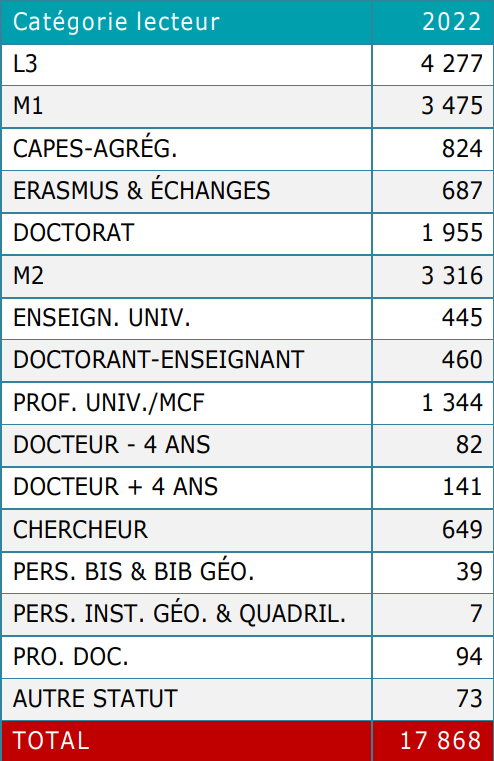
\includegraphics[width=2.56806in,height=3.98889in]{vertopal_157ae480aa4a4b07be198b586a812241/media/image25.png}
	\caption{Profil des lecteurs fréquentant la BIS}
\end{table}

Le tableau ci-dessus renseigne sur le niveau d'étude des lecteurs qui fréquentent la bibliothèque. À la date du 31 décembre 2022, la BIS comptait au total 17 868 lecteurs selon le rapport d'activité de 2022\footnote{« Rapport d’activité 2022 de la BIS », Bibliothèque interuniversitaire de la Sorbonne, p. 42. \url{https://www.bis-sorbonne.fr/biu/IMG/pdf/bis_ra_2022_web.pdf}.}. Nous constatons que la majorité des lecteurs de la BIS sont donc des étudiants ayant un niveau Bac + 3 au minimum, le reste étant des chercheurs, doctorants et enseignants. La question ici est donc de savoir si ces lecteurs sont représentatifs des utilisateurs de la bibliothèque numérique (NuBIS) qui sont eux le public concerné par l'implémentation de l'OCR. Bien que l'accès à NuBIS ne nécessite pas de carte lecteur, nous pouvons tout de même supposer que les deux publics sont proches, les utilisateurs de NuBIS penchant probablement plus vers le groupe des chercheurs dû à sa collection patrimoniale et tournée vers la recherche comme nous le verrons par la suite.

\section{Organisation de la bibliothèque}

La Bibliothèque interuniversitaire s'organise dans un premier temps autour de cinq départements : \\

\begin{itemize}
	\item
	\begin{quote}
		\textbf{Département de l'accueil des publics et de la communication des documents} : Il est chargé d’organiser et de garantir l’accès des lecteurs aux espaces et aux ressources de la bibliothèque. Il élabore et met en œuvre le règlement de la bibliothèque à destination du public.
	\end{quote}
	\item
	\begin{quote}
		\textbf{Département du traitement documentaire
		} :
		Il a pour mission principale, au sein de la BIS, le catalogage de tous les documents des collections du fonds général de la bibliothèque, ainsi que des e-books acquis de façon pérenne.
	\end{quote}
	\item
	\begin{quote}
		\textbf{Le département du développement des collections
		} :
		Il a pour fonctions de développer les collections du fonds général en mettant en œuvre la politique documentaire définie par la bibliothèque, en particulier dans les domaines prioritaires des collections (Antiquité, Histoire, Philosophie et Littérature).
	\end{quote}
	\item
	\begin{quote}
		\textbf{Le département des Manuscrits et des livres anciens} : Il assure la gestion des collections patrimoniales de la bibliothèque. Il est question ici des manuscrits, estampes et autres documents iconographiques, livres imprimés avant 1801, ouvrages à caractère bibliophilique des XIX\textsuperscript{e} et XX\textsuperscript{e} siècles, auxquels s’ajoutent les thèses dactylographiées et certaines thèses imprimées.
	\end{quote}
	\item
	\begin{quote}
		\textbf{Bibliothèque de géographie
		} : Elle constitue elle aussi un département de la BIS. Elle traite toutes les collections géographiques et mène des actions spécifiques visant à la mise en valeur de ses fonds. Elle est liée par son fonctionnement à l’Institut de géographie. \\
	\end{quote}
\end{itemize} 

En plus de ces cinq départements, il existe à la Sorbonne quatre services transversaux impliqués dans le fonctionnement de la bibliothèque et qui travaillent avec l'ensemble des départements : \\

\begin{itemize}
	\item
	\begin{quote}
		\textbf{Service des moyens généraux
		} : Il est chargé du traitement de toutes les questions administratives. Il traite avec les services centraux de l’Université Paris 1 Panthéon-Sorbonne, avec les services du ministère chargé de l’enseignement supérieur ainsi qu’avec le rectorat.
	\end{quote}
	\item
	\begin{quote}
		\textbf{Service de l'informatique et des systèmes d'information} :
		Il assure le traitement de toutes les questions liées à l’informatique de la bibliothèque.
	\end{quote}
	\item
	\begin{quote}
		\textbf{Service de la conservation et de la gestion matérielle des collections} : Il traite des questions liées à la conservation, à la préservation des collections, à l’implantation et au suivi des exemplaires de monographies et de périodiques.
	\end{quote}
	\item
	\begin{quote}
		\textbf{Service de la valorisation numérique des collections et du soutien à la recherche (SERVAL)
		} : Il s’agit du service au sein duquel notre stage s’est déroulé. Il a pour mission de définir, coordonner et opérer des actions de valorisation des collections sur des outils numériques, ainsi que promouvoir et porter des partenariats scientifiques en lien avec des projets de recherche. Le SERVAL gère donc la bibliothèque numérique NUBIS et coordonne le projet d’OCR dont il est question dans cette étude. 
	\end{quote}
\end{itemize} 


\section{La bibliothèque numérique}

En 1978, la Sorbonne voit l'installation d'un atelier de microfilmage au sein de sa bibliothèque. Cette date marque les débuts timides d'une politique de reproduction des collections physiques qui aboutiront quatre décennies plus tard à la naissance de sa bibliothèque numérique NuBIS. Ce cheminement s'est en effet inscrit dans un paysage documentaire bouleversé à partir du milieu des années 1990 par l'arrivée de l'Internet et le développement des nouvelles technologies puis par la généralisation des programmes de numérisation au sein des bibliothèques de l'enseignement supérieur. \footnote{Bobis, Laurence, et Boris Noguès. \emph{La Bibliothèque de la Sorbonne, 250 ans d’histoire au cœur de l’Université}. Éditions de la Sorbonne. Paris, France, 2022. p. 257.} C'est dans ce contexte que la BIS a installé en février 2007 son
propre atelier de numérisation qui est équipé d'un scanner Digibook 10 000 RGB conçu par la société i2S. Celui-ci est adapté au traitement des
documents qui peuvent être anciens et fragiles, et permet une numérisation en haute définition\footnote{Bibliothèque
	numérique de la Sorbonne. « Aspects techniques ». Consulté le 9 août
	2024.
	\url{https://nubis.bis-sorbonne.fr/page/aspects-techniques}.}. À partir de cette date, la numérisation en couleur devient la règle avec la production de fichiers au format jpeg compressé à 50\% et au format tiff qui lui reste non compressé. \\

Cependant, au début des années 2010, alors qu'elle était pionnière dans le paysage documentaire universitaire en se dotant assez tôt d'un tel équipement de pointe qui est adapté à la numérisation des documents patrimoniaux, la BIS n'a pas encore été en mesure de réaliser le volet informatique du projet de numérisation des sources de l'histoire de l'université. Ce projet avait été élaboré en 2004 et devait déboucher sur la diffusion des données numérisées. \footnote{Bobis, Laurence, et Boris Noguès. \emph{La Bibliothèque de la Sorbonne, 250 ans d’histoire au cœur de l’Université}. Éditions de la Sorbonne. Paris, France, 2022. p. 267.} Après le retour de la BIS dans ses locaux historiques à la Sorbonne, les réflexions autour de la diffusion des documents numérisés reprennent en 2014. \\

Deux pistes différentes sont alors envisagées, ces pistes ayant déjà été explorées par d'autres bibliothèques interuniversitaires. La première fait appel à la solution « Gallica Marque blanche »\footnote{
	\url{https://www.bnf.fr/fr/gallica-marque-blanche}.}, dont la bibliothèque nationale et interuniversitaire de Strasbourg a été la première à adopter pour la mise en ligne de sa bibliothèque numérique Numistral. Il s'agit d'un dispositif de coopération numérique qui s’adresse aux établissements ayant numérisé ou souhaitant numériser une partie de leurs collections, mais qui ne disposent pas de plateforme en ligne qui soit capable de diffuser ces collections numérisées. Cette option serait alors la moins coûteuse pour la BIS. Cependant, elle comporte des limites du point de vue de la valorisation des collections. Ces limites sont causées par le rôle pivot joué par les catalogues de la BnF (Bibliothèque nationale de France) dans le dispositif. En effet, lorsqu'une édition imprimée est déjà signalée dans le catalogue général de la BnF, c'est la notice de ce catalogue qui sert de sources aux métadonnées descriptives qui accompagnent le document, sans la possibilité de les compléter par les donnée propres à l'exemplaire reproduit (la reliure, la présence d'annotations manuscrites...).
 \\
 
 La seconde piste consistait à faire appel à des prestataires externalisés qui permettrait à la BIS de développer sa propre bibliothèque numérique. Le coût d'une telle prestation est estimé alors à 100 000 euros. Compte tenu des difficultés budgétaires auxquelles la Sorbonne se trouve alors confrontée, cette piste est abandonnée elle aussi. Finalement, c'est une solution moins onéreuse reposant sur l'utilisation du logiciel libre Omeka qui est adoptée. Celle-ci est réputée pour sa prise en main aisée et a déjà été choisie par plusieurs bibliothèques de l'enseignement supérieur. Le projet de la mise en place de la bibliothèque numérique a été réalisé en
2016 par Mylène Ravereau, étudiante en master « Technologies numériques
appliquées à l'histoire », dans le cadre de son stage de fin d'études à
l'École nationale des chartes. Ce projet s'est déroulé
sous la supervision conjointe du Département des manuscrits et des
livres anciens et du Service de l'informatique et des systèmes
d'information\footnote{Bibliothèque numérique de la
	Sorbonne. « Équipe ». Consulté le 9 août 2024.
	\url{https://nubis.bis-sorbonne.fr/page/equipe}.}. \\ 

Il fallait ensuite s'assurer de la diffusion et de la pérennisation des données, de paramétrer l'application et d'intégrer les données numérisées sur Omeka. Cette intégration a nécessité le renommage systématique des fichiers suivant un plan de nommage conforme aux préconisations de la norme ISO 9660, leur conversion aux formats de diffusion qui sont requis (jpeg et pdf) ainsi que la création de métadonnées respectant le guide d'interopérabilité rédigé par la BnF sur le protocole OAI-PMH\footnote{
	\url{https://www.bnf.fr/sites/default/files/2019-02/Guide_oaipmh.pdf}.}. \\

La bibliothèque numérique NuBIS a finalement été inaugurée le 25 avril 2017 avec plus de 40 000 images
provenant de la numérisation d'environ 1 000 documents issus des fonds
patrimoniaux de la bibliothèque.\footnote{Bobis, Laurence, et Boris Noguès. \emph{La Bibliothèque de la Sorbonne, 250 ans d’histoire au cœur de l’Université}. Éditions de la Sorbonne. Paris, France, 2022. p. 269.} Début 2024, elle rassemble plus de 11
000 documents, totalisant plus de 450 000 images. NuBIS est
régulièrement enrichie au fil de l'année par la
numérisation de nouveaux documents patrimoniaux conservés à la
Bibliothèque interuniversitaire de la Sorbonne.\footnote{Bibliothèque
	numérique de la Sorbonne. « Corpus numérisés ». Consulté le 9 août
	2024.
	\url{https://nubis.bis-sorbonne.fr/page/le-corpus}.}
La bibliothèque numérique est aujourd'hui encore gérée par l'intermédiaire du logiciel Omeka
S qui a succédé à Omeka\footnote{« Omeka S ». Consulté le 9 août 2024.
	\url{https://omeka.org/s/}.} tandis que
les images sont hébergées sur le visualiseur IIIF Mirador\footnote{«
	Mirador --- Home ». Consulté le 9 août 2024.
	\url{https://projectmirador.org/}.}. Elle est hébergée sur un serveur de l'université Paris 1 Panthéon-Sorbonne qui relève du département du Système d'information et des usages numériques (DSIUN). \\

La Sorbonne a par ailleurs fait le choix de placer les données de sa bibliothèque numérique sous une licence ouverte conçue par Etalab tout en préservant son service de numérisation à la demande qui lui est payant. En outre, dans la perspective d'une politique de numérisation plus large, la gestion et la coordination de ce nouvel outil ont été confiées à une nouvelle mission nommée « Valorisation des collections et soutien à la recherche ». Cette mission a ensuite été renforcée au point de devenir un service à part entière sous le nom de « Service de la valorisation numérique des collections et du soutien à la recherche  » (SERVAL) évoqué précédemment. \\ 

\begin{figure} [H]
	\centering
	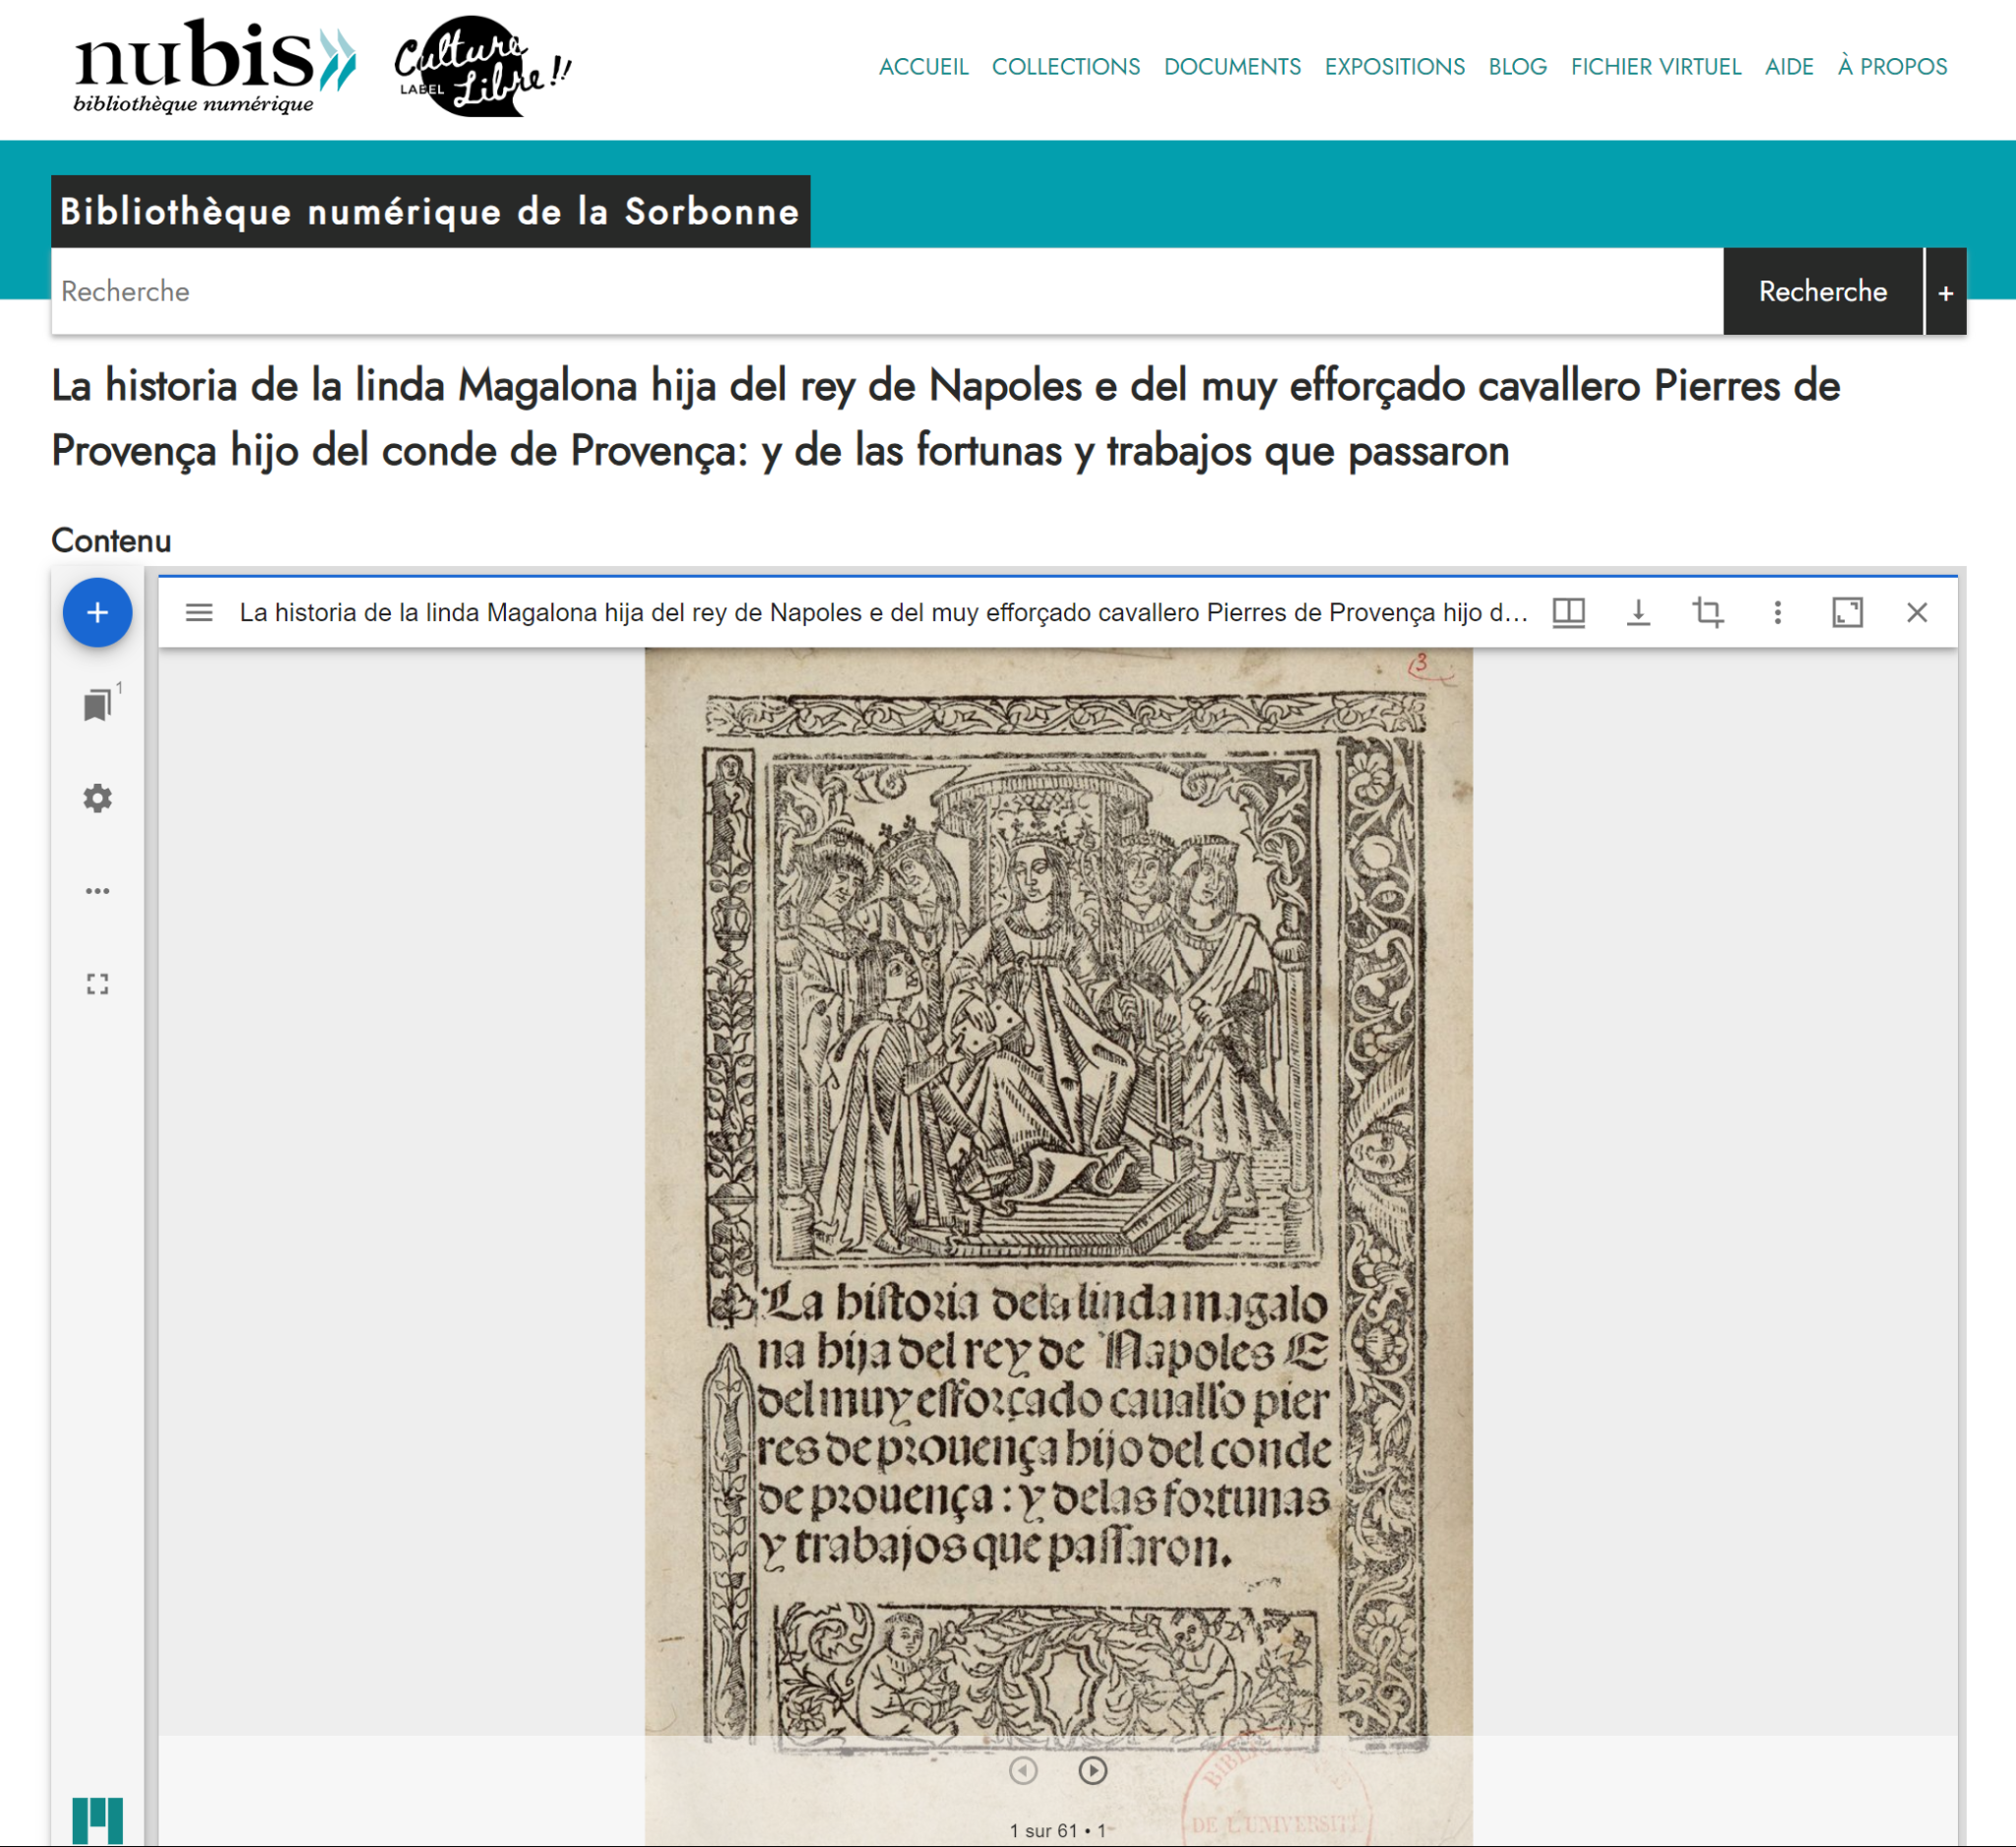
\includegraphics[width=5.23681in,height=4.77569in]{vertopal_157ae480aa4a4b07be198b586a812241/media/image1.png}
	\caption{Capture d'écran de l'interface de NuBIS avec Mirador}
\end{figure}

\begin{figure} [H]
	\centering
	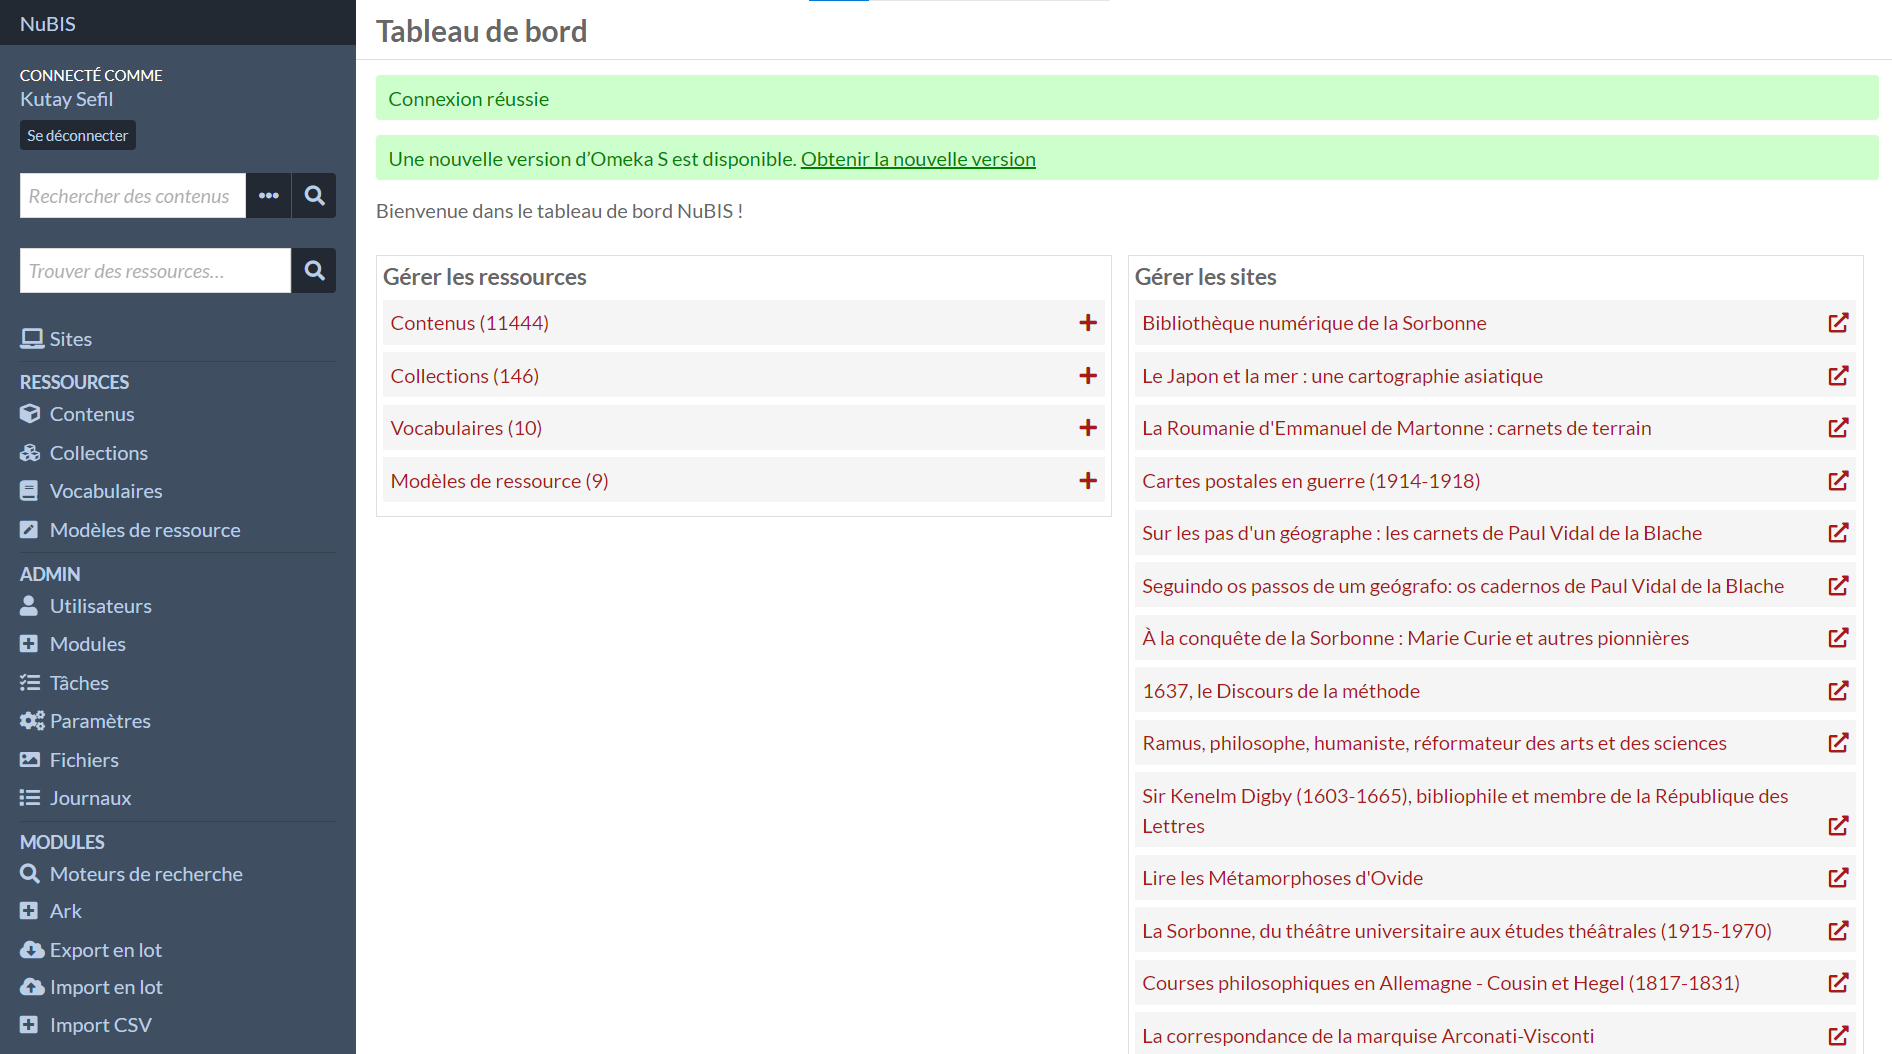
\includegraphics[width=6.4in,height=3.6in]{vertopal_157ae480aa4a4b07be198b586a812241/media/image26.png}
	\caption{Capture d'écran de l'interface d'Omeka S}
\end{figure}



Des efforts considérables ont été effectués par la suite afin d'améliorer la visibilité de NuBIS, par exemple avec la création systématique de liens pointant vers la bibliothèque numérique depuis les notices se trouvant les catalogues collectifs comme Sudoc pour les imprimés ou Calames pour les manuscrits. Un autre exemple est la mise en place d'expositions virtuelles qui reprennent le plus souvent les contenus des expositions présentées dans les murs de la bibliothèque avec la participation d'enseignants-chercheurs. Une stratégie de valorisation plus large visant une communication à travers les réseaux sociaux et un enrichissement de Wikipédia a aussi été initiée. Plus important encore, NuBIS est désormais moissonnée par Gallica grâce à la mise en place d'un entrepôt OAI, ainsi que par le moteur de recherche Isidore (spécialisé dans le domaine des sciences humaines et sociales) et enfin par le portail Biblissima (spécialisé dans le patrimoine écrit du Moyen Âge et de la Renaissance en Occident). \footnote{Bobis, Laurence, et Boris Noguès. \emph{La Bibliothèque de la Sorbonne, 250 ans d’histoire au cœur de l’Université}. Éditions de la Sorbonne. Paris, France, 2022. p. 271.}  \\


Les collections disponibles sur NuBIS sont donc issues d'un chantier de
numérisation des collections patrimoniales mené depuis une quinzaine
d'années. À la rentrée universitaire 2017, le chantier d'alimentation initiale qui consistait à traiter de manière rétrospective l'ensemble des données libres de droits accumulées depuis le début des activités de numérisation internes à la bibliothèque a été quasiment achevé. Désormais, les travaux de reproduction nouvellement effectués par l'atelier de numérisation sont versés et publiés au fil de l'eau sur NuBIS. \\

La politique de numérisation de la bibliothèque est aujourd'hui définie par le Département des manuscrits et des livres anciens. Elle consiste à numériser les livres rares et
les unica de la collection de la BIS c'est-à-dire les
livres dont un seul exemplaire est répertorié dans le catalogue Sudoc.
Les points forts sont concentrés essentiellement sur l'histoire de
l'université à Paris dans toutes les périodes de son histoire et sous
tous ses aspects : institution, pédagogie, enseignants, vie étudiante,
bâtiments, notamment par la diffusion des archives de
l'Université de Paris et des archives de la bibliothèque
de la Sorbonne. On y retrouve aussi des numérisations en lien avec les
projets de recherche et les expositions, mais dans une quantité bien
moindre. Un changement dans cette politique est prévu avec
l'introduction d'un marché de numérisation
l'an prochain\footnote{D'après un échange avec Cécile
	Obligi et Laurie Aoustet, conservatrices à la BIS.} mais à l'heure
actuelle, la numérisation s'organise autour de neuf collections en plus
des collections invitées qui sont hébergées dans la bibliothèque numérique mais ne sont pas issues des
collections conservées à la BIS\footnote{Bibliothèque numérique de la
	Sorbonne. « Corpus numérisés ». Consulté le 9 août 2024.
	\url{https://nubis.bis-sorbonne.fr/page/le-corpus}.}
: \\

\begin{itemize}
	\item
	\begin{quote}
		Les sources de l'histoire de l'Université de Paris mentionnées précédemment qui regroupe des
		documents relatifs à l'évolution des bâtiments de l'Université et des
		collèges qui lui étaient rattachés ainsi qu'aux enseignements qui y
		étaient dispensés.
	\end{quote}
	\item
	\begin{quote}
		Des documents manuscrits, imprimés et iconographiques dédiés à
		l'histoire de la bibliothèque et mis en ligne à l'occasion du 250e
		anniversaire de la BIS.
	\end{quote}
	\item
	\begin{quote}
		Des manuscrits médiévaux hérités des bibliothèques médiévales de
		plusieurs collèges parisiens.
	\end{quote}
	\item
	\begin{quote}
		Des papiers d'universitaires et d'érudits qui valorisent les documents
		des fonds comme ceux de Léon Chestov ou encore de la marquise
		Arconati-Visconti.
	\end{quote}
	\item
	\begin{quote}
		Des cartes postales sous forme de caricatures de la Première Guerre mondiale.
	\end{quote}
	\item
	\begin{quote}
		Des cartes géographiques rares allant du XVI\textsuperscript{e} au
		XIX\textsuperscript{e} siècles.
	\end{quote}
	\item
	\begin{quote}
		Des imprimés et manuscrits de l'école française de géographie.
	\end{quote}
	\item
	\begin{quote}
		Des manuscrits philosophiques clandestins du XVIII\textsuperscript{e}
		siècle.
	\end{quote}
	\item
	\begin{quote}
		Depuis mai 2024, « Matrimoine » qui est une collection d'écrits de
		femmes ou d'images témoignant de la présence des femmes à
		l'université. \\
	\end{quote}
\end{itemize}

NuBIS se positionne donc dans le paysage foisonnant des bibliothèques numériques d'aujourd'hui avec des atouts considérables. Elle fait face aux nouveaux enjeux que représente la valorisation des collections par la recherche. Grâce à sa politique de numérisation structurée, elle s'engage à soutenir des projets de recherche en prenant appui sur ses collections. Outre une organisation sous forme de collection, les documents en ligne sur NuBIS peuvent être distingués selon  les catégories
suivantes qui renseignent sur leur type : manuscrits, monographies imprimées, cartes postales,
photographies, documents cartographiques, estampes, dessins, et enfin
tapuscrits. Le diagramme ci-dessous montre la répartition des documents
sur NuBIS en fonction de leur type : \\

\begin{figure} [H]
	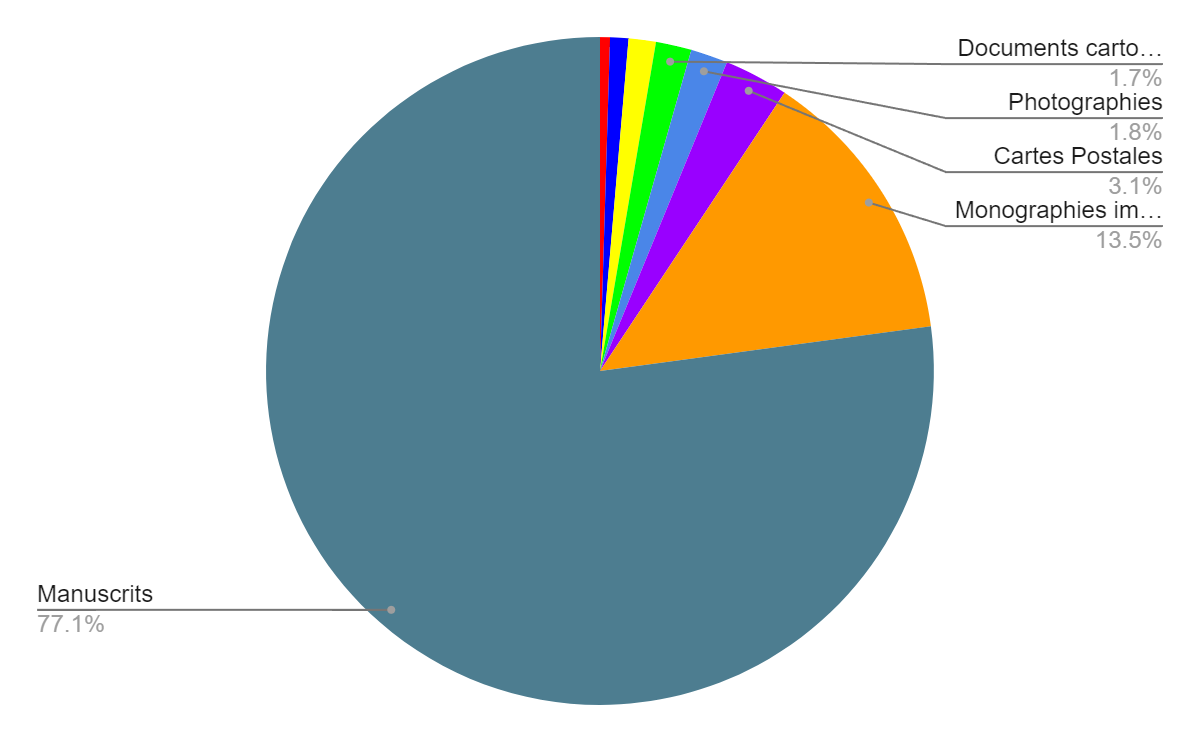
\includegraphics[width=5.83194in,height=3.60972in]{vertopal_157ae480aa4a4b07be198b586a812241/media/image2.png}
	\caption{Répartition des documents par type sur NuBIS}
\end{figure}

Par définition, la reconnaissance optique de caractères (OCR) concerne
uniquement les documents imprimés. Ainsi, nous nous intéresserons ici
uniquement aux monographies imprimées (en orange) ainsi qu'aux
tapuscrits (en rouge), ce qui représente environ 1500 documents soit
14\% de l'ensemble des documents sur NuBIS. Il convient donc à présent
de nous intéresser plus en détail à cette collection afin d'étudier la
qualité attendue de l'OCR sur cet ensemble de documents. Pour cela, nous
avons jugé pertinent d'établir une typologie de ces imprimés et
tapuscrits selon leurs caractéristiques matérielles et typographiques,
lesquelles peuvent influer sur la qualité de l'OCR et donc sur le choix
du logiciel d'OCR. 

\section{Typologie des documents à océriser}

En ce qui concerne les tapuscrits tout d'abord, il en existe
actuellement 52 sur NuBIS dont 33 sont des lettres dactylographiées du
début du XX\textsuperscript{e} siècle adressées à la marquise
Arconati-Visconti, similaires entre elles et présentant une impression
de bonne qualité. De son nom de naissance Marie Peyrat (1840-1923), elle
est la fille de l'homme de lettres Alphonse Peyrat, journaliste
républicain devenu après 1870 député puis sénateur. En 1873, elle
devient par mariage la marquise Arconati-Visconti. Son mari, le jeune
Giammartino, issu d'une des plus grandes familles
italiennes et propriétaire de nombreuses propriétés à travers
l'Europe, décède trois ans plus tard sans laisser
d'héritier, léguant à la nouvelle marquise une immense
fortune. Elle utilise cet héritage pour entretenir ses résidences,
devenir une mécène, mais surtout pour soutenir la jeune République qui
voit le jour en France en 1870 dans les domaines de
l'art et des savoirs. Passionnée par
l'histoire et la politique, dreyfusarde, Marie
Arconati-Visconti réunit autour de sa table les principaux acteurs de la
Troisième République : députés, ministres, hauts fonctionnaires, ainsi
que des savants et professeurs du Collège de France, de
l'École des chartes et de l'École des
hautes études\footnote{DERROT, Sophie. « La marquise Arconati Visconti
	», 22 novembre 2023.
	\url{http://blog.bibliotheque.inha.fr/fr/posts/marquise_arconati_visconti.html}.}.
Ses correspondances entretenues avec ces figures notables de la
Troisième République ont été numérisées après un chantier d'un an et
mises en ligne sur NuBIS en décembre 2019.\footnote{L'ensemble des
	correspondances manuscrites et tapuscrites se trouvent ici :
	\url{https://nubis.bis-sorbonne.fr/ark:/15733/ffzf}.}
Elles ont par ailleurs donné lieu à dans le cadre d'une exposition
virtuelle.\footnote{Site de l'exposition virtuelle :
	\url{https://nubis.bis-sorbonne.fr/web/marquise-arconati-visconti/accueil.html}.} \\

Les autres tapuscrits ont une typographie très lisible eux aussi car ils sont
exempts de toute lettre ou caractère archaïque puisque les machines à
écrire sont une invention relativement récente, datant de la fin du
XIX\textsuperscript{e} siècle\footnote{Cortada, James W. \emph{Before
		the Computer: IBM, NCR, Burroughs, and Remington Rand and the Industry
		They Created, 1865-1956}. Princeton University Press, 2015. p. 38.}.
Cependant, les tapuscrits présentent parfois un problème particulier ce
type de support : les caractères imprimés au verso sont lisibles au
recto et vice-versa, ce qui peut causer des difficultés de lecture à un
logiciel d'OCR. Hormis ce point, la qualité visuelle des tapuscrits en
ligne sur NuBIS ne pose pas de difficulté pour l'OCR avec une
typographie qui est visuellement très proche d'un tapuscrit à l'autre. \\

\begin{figure} [H]
	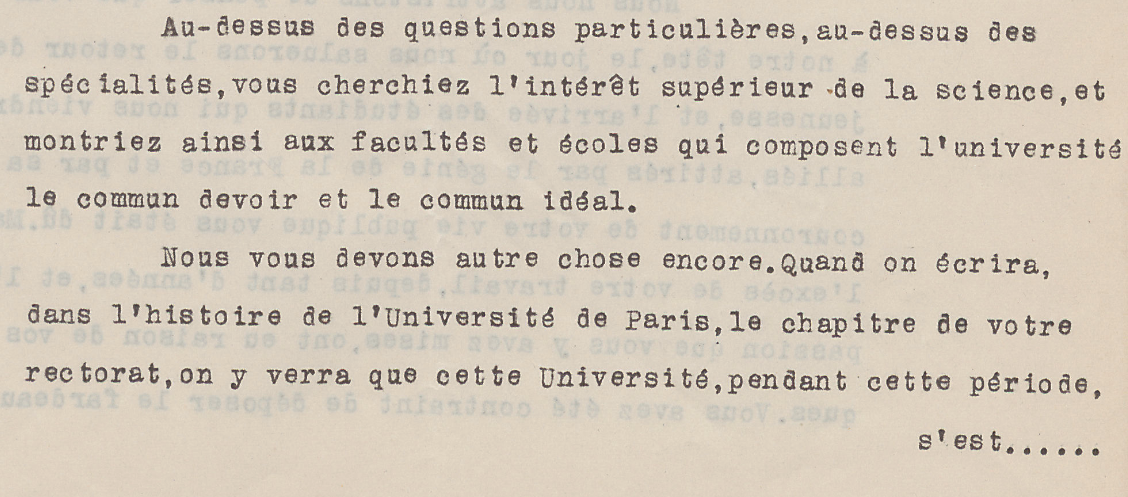
\includegraphics[width=6.2806in,height=2.76389in]{vertopal_157ae480aa4a4b07be198b586a812241/media/image3.png}
	
	\caption{Exemple de tapuscrit avec le texte au verso lisible
	(\url{https://nubis.bis-sorbonne.fr/ark:/15733/9qp6?mirador-1=1})}
\end{figure}


Quant aux monographies imprimées, elles sont bien plus nombreuses sur
NuBIS puisque nous en dénombrons plus de 1400 en ligne actuellement.
Cette collection d'imprimés est ancienne et a une provenance
universitaire : son noyau d'origine provient d'établissements
d'enseignement et d'anciens professeurs. On peut dès le début
présupposer que la précision de l'OCR sera très variable elle aussi
puisqu'elle va dépendre des caractéristiques du matériel source qui sont
mentionnés dans le rapport sur l'OCR du consortium IMPACT et que nous
avons rappelé dans notre introduction\footnote{Anderson, Niall, Gunter
	Muhlberger, et Apostolos Antonacopoulos. « Optical Character
	Recognition - IMPACT Best Practice Guide ». \emph{Optical Character
		Recognition}, 2023. p. 8-11.
	\url{https://www.digitisation.eu/wp-content/uploads/2023/09/OpticalCharacterRecognition-IBPG_01.pdf}.}.
Ceux-ci sont en effet liés à l'aspect matériel de l'ouvrage en lui-même
puisque la qualité de la numérisation est excellente sur NuBIS quelle
que soit la date de publication de l'ouvrage avec des images de très
haute définition en termes de pixels. Pour cette raison, il est
nécessaire de distinguer tout d'abord les monographies imprimées en
plusieurs grandes catégories avant d'ensuite étudier les particularités
des ouvrages qui peuvent causer des difficultés pour l'OCR. \\

Il a été envisagé dans un premier temps d'effectuer une typologie par
type d'imprimé : lettres, actes, thèses, pièces de
théâtre, ouvrages scientifiques... Or, pour un même type
d'imprimé, la qualité de l'OCR
n'est pas la même en fonction de la date du document, la
qualité de l'impression et les autres caractéristiques
typographiques. Par conséquent, il nous a paru plus pertinent d'établir
une typologie de nature chronologique, fondée sur la date de publication
des documents. En effet, malgré les particularités propres à chaque
ouvrage, nous avons observé qu'un découpage par période traduit assez
bien l'évolution de la qualité de l'OCR pour la collection des imprimés
: plus ces documents sont récents, meilleure est la qualité de l'OCR.
Nous avons donc effectué un découpage chronologique en quatre périodes
distinctes, chacune étant caractérisée par des éléments typographiques
qui lui sont caractéristiques ou du moins plus récurrents que dans les
ouvrages des autres périodes. Ce découpage a été validé par la
responsable de la Réserve de la bibliothèque. 

Les graphiques suivants montrent respectivement la répartition des
imprimés par décennie et par siècle sur NuBIS : \\

\begin{figure} [H]

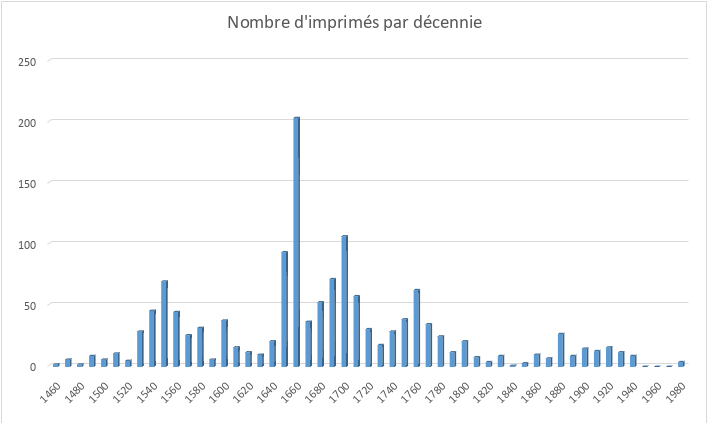
\includegraphics[width=5.82431in,height=3.34861in]{vertopal_157ae480aa4a4b07be198b586a812241/media/image4.png}

\caption{Répartition du nombre d'imprimés par décennie}

\end{figure}

\begin{figure} [H]
	
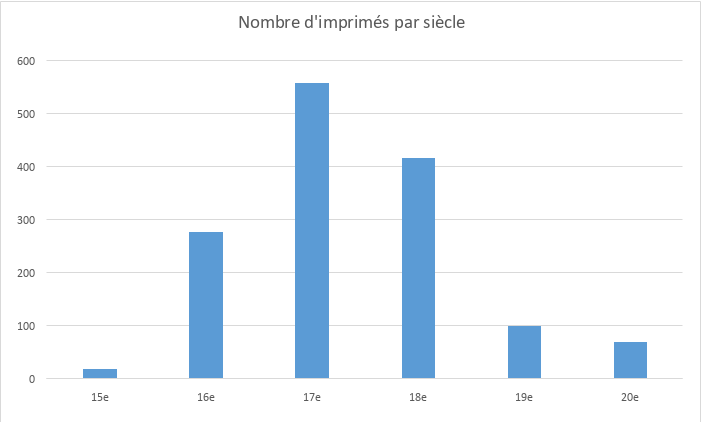
\includegraphics[width=5.82403in,height=3.36667in]{vertopal_157ae480aa4a4b07be198b586a812241/media/image5.png}

\caption{Répartition du nombre d'imprimés par décennie}

\end{figure}

\subsection{1467 - 1539}

Cette période comprend l'intégralité des incunables et une partie des
documents du XVI\textsuperscript{e} siècle. La date de 1467 correspond
au plus ancien document imprimé qu'on trouve sur NuBIS\footnote{Gerson,
	Jean, et Ulrich Zell. \emph{Conclusiones de diversis materiis
		moralibus, sive De regulis mandatorum}. Köln, France: Ulrich Zell,
	1467.
	\url{https://nubis.bis-sorbonne.fr/ark:/15733/nkd1}.},
tandis que celle de 1539 correspond au dernier ouvrage en écriture
gothique actuellement disponible sur NuBIS\footnote{« Das Vater Unser
	kurz ausgelegt/ und inn Gesang weyse gebracht durch D. Mar. Luth. »
	Consulté le 12 août 2024.
	\url{https://nubis.bis-sorbonne.fr/ark:/15733/4frd}.}.
La présence d'incunables rares au sein de la BIS et de sa bibliothèque
numérique n'est pas surprenante puisque l'apparition de l'imprimerie en
France naît d'une volonté de l'Université de Paris de posséder des
exemplaires de livres en nombre\footnote{Barbier, Frédéric. « Chapitre 2. Gutenberg et l'invention de l'imprimerie ». \emph{Histoire du livre en Occident}. Armand Colin, 2020. p. 114.}.
Plus précisément, ce sont Guillaume Fichet et Jean Heynlin, condisciples
à l'Université de Paris, qui sont à l'origine du premier
livre imprimé en France en 1470 (les \emph{Epistolae} de Gasparin de
Bergame).\footnote{Veyrin-Forrer, Jeanne. «\,Hommage aux premiers
	imprimeurs de France. 1470-1970\,», \emph{Bulletin des bibliothèques
		de France (BBF)}, 1971, n° 2, p. 65-80.
	\url{https://bbf.enssib.fr/consulter/bbf-1971-02-0065-001}} \\

Ainsi, cette tranche chronologique est composée majoritairement
d'ouvrages en écriture gothique, ce qui est dans la continuité des manuscrits médiévaux gothiques du Moyen Âge tardif. Cette graphie représente un
défi considérable pour l'ensemble des moteurs d'OCR. Par exemple,
Gallica (la bibliothèque numérique de la Bibliothèque nationale de France)
ne propose pas d'OCR pour les documents de cette période. De manière
générale, la grande majorité des ouvrages de cette période est en latin,
le reste étant en moyen français, espagnol, allemand et grec. Toujours dans la continuité de l'époque médiévale, le latin continue donc à dominer largement les écrits mais cette dominations tend à s'affaiblir avec l'invention de l'imprimerie au profit des langues vernaculaires comme le français : nous passons de 97\% de titres en latin en 1467 à 74\% en 1477 puis 65\% en 1492.\footnote{Barbier, Frédéric. « L’invention de l’imprimerie et l’économie des langues en Europe au XVe siècle ». \emph{Histoire et Civilisation Du Livre} 4 (2008): p. 21‑46.}. Comme l'ont montré les graphiques précédents, les ouvrages de cette période constituent seulement une
très petite partie des imprimés en ligne sur NuBIS. \\

\begin{figure} [H]
	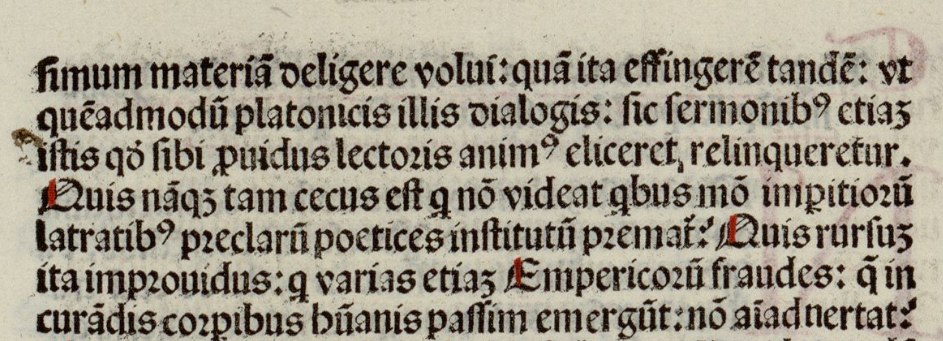
\includegraphics[width=6.26806in,height=2.26389in]{vertopal_157ae480aa4a4b07be198b586a812241/media/image6.png}
	
	\caption{Extrait d'un ouvrage de la fin du
		XV\textsuperscript{e} siècle.
		(\url{https://nubis.bis-sorbonne.fr/ark:/15733/ng7n?mirador-1=4})}
\end{figure}

Nous pouvons observer ici une graphie gothique typique des imprimés de cette période. L'ouvrage est en latin comme c'est le cas encore une fois pour la plupart des imprimés de l'époque. Nous remarquons aussi la présence de nombreuses abréviations sous la forme de caractères spéciaux, ce qui peut compliquer le travail de l'OCR. Le papier rend ce travail d'autant plus difficile puisque le l'encre et le texte de la page au dos sont visibles ici. Enfin, les majuscules et lettrines sont en rouge et donc dans une couleur différente du reste du texte, ce qui peut impacter la qualité de l'OCR là aussi. 


\subsection{1539 - fin du XVII\textsuperscript{e} siècle}

Les ouvrages du reste du XVI\textsuperscript{e} siècle et du
XVII\textsuperscript{e} siècle ont été regroupés au sein d'une même
catégorie. Ceux-ci constituent environ la moitié de la collection des
monographies imprimées de la NuBIS. Ces monographies sont caractérisées
par une qualité d'impression souvent médiocre et des particularités
récurrentes : présence d'annotations manuscrites, caractères peu
lisibles, courbure du texte, abondance de l'écriture italique. De plus,
l'expansion rapide de l'imprimerie en Europe à cette période a donné
lieu au développement de nombreuses polices de caractères, chaque
imprimerie utilisant ses propres caractères mobiles\footnote{Heil,
	Jacob, et Todd Samuelson. « Book History in the Early Modern OCR
	Project, or, Bringing Balance to the Force ». \emph{Journal for Early
		Modern Cultural Studies} 13, n\textsuperscript{o} 4 (2013): p.
	90‑103.\url{https://www.jstor.org/stable/jearlmodcultstud.13.4.90}.}. En France, nous pouvons citer Claude Garamond, l'un des premiers graveurs et fondeurs typographiques indépendants du royaume, qui produit des fontes romaines et italiques employées par Robert Estienne à partir des années 1540\footnote{Barbier, Frédéric. « Chapitre 4. L'Ancien Régime : formes de l'imprimé ». \emph{Histoire du livre en Occident}. Armand Colin, 2020. p. 239.}. \\

Cette multitude de polices de caractères influent ainsi de manière négative sur les performances des outils
d'OCR. Environ les trois quarts des ouvrages de cette tranche
chronologique sont en latin et un quart en français. Pourtant, l'historien du livre Henri-Jean Martin a montré que l'équilibre entre le latin et le français s'inversait déjà en faveur de cette dernière dans la décennie 1560\footnote{« Chapitre 2. Le paradigme de l'absolutisme : l'Europe classique et l'imprimé ». \emph{Ibid}., p. 197.}. La domination du latin au sein des imprimés de la BIS encore à cette période peut s'expliquer par l'abondance des imprimés universitaires et religieux où la langue latine restait la référence. Les exemples
ci-dessous, pris dans la période concernée, illustrent des cas
récurrents susceptibles de diminuer la qualité de l'OCR.

\begin{figure} [H]
	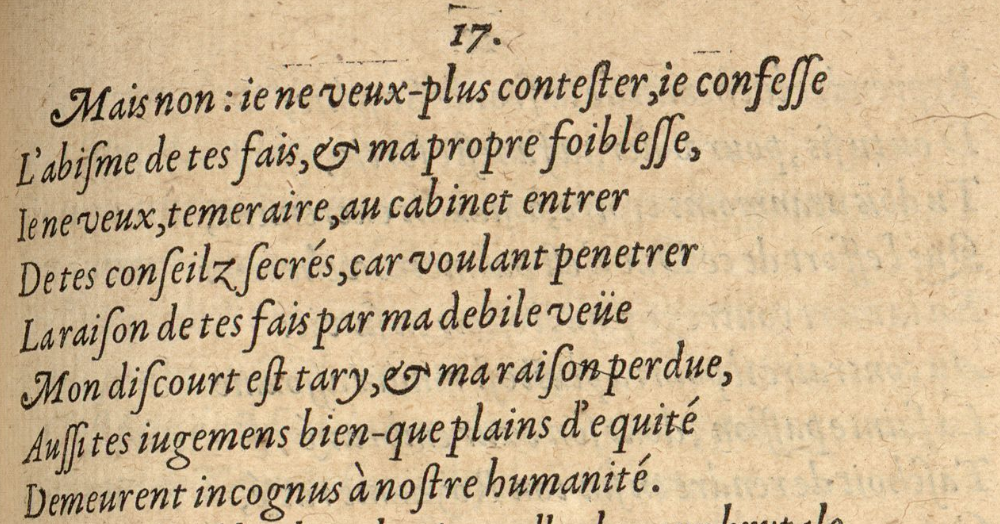
\includegraphics[width=6.26806in,height=3.27778in]{vertopal_157ae480aa4a4b07be198b586a812241/media/image7.png}
	\caption{Extrait d'un ouvrage du début XVII\textsuperscript{e}
		siècle.
		(\url{https://nubis.bis-sorbonne.fr/ark:/15733/49bk?mirador-1=17})}
\end{figure}

Dans l'extrait ci-dessus, le texte en italique et la courbure de la page sur le côté gauche diminuent grandement
la lisibilité du texte. L'espacement des mots est lui aussi difficile à identifier à certains moments et le texte au dos de la page ressort encore une fois.\\



\begin{figure} [H]
	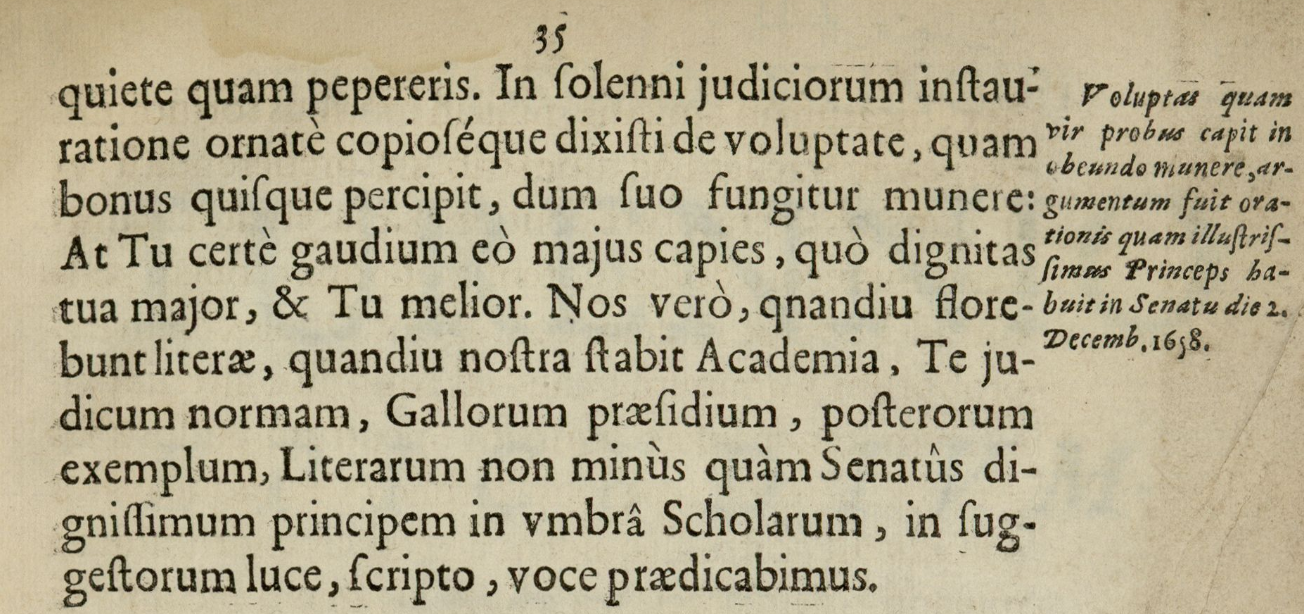
\includegraphics[width=6.26806in,height=2.94444in]{vertopal_157ae480aa4a4b07be198b586a812241/media/image8.png}
	\caption{Extrait d'un ouvrage du milieu du XVII\textsuperscript{e}
		siècle.
		(\url{https://nubis.bis-sorbonne.fr/ark:/15733/1khm?mirador-1=43})}
\end{figure}

Dans cet exemple, nous remarquons la présence d'un texte en italique situé en marge sur le côté droit, compliquant ainsi la
segmentation de la page. En outre, ces notes en italique sont peu lisibles dû à leur petite taille. \\


\begin{figure} [H]
	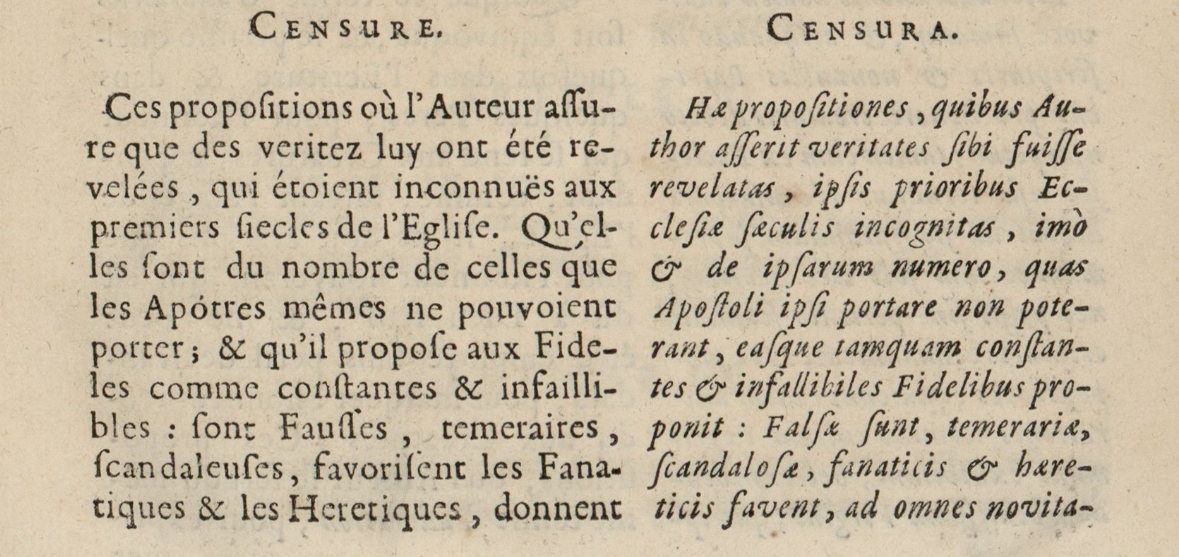
\includegraphics[width=6.13056in,height=2.89236in]{vertopal_157ae480aa4a4b07be198b586a812241/media/image9.png}
	\caption{Extrait d'un ouvrage de la fin du XVII\textsuperscript{e}
		siècle.
		(\url{https://nubis.bis-sorbonne.fr/ark:/15733/17zw?mirador-1=7})}
\end{figure}

Enfin, nous pouvons voir ici un exemple de texte réparti sur deux colonnes au sein d'une même page. Non seulement les styles sont différents (romain et italique), mais les langues le sont aussi (français et latin). Cela complique à la fois la segmentation de la page et la lecture des caractères. 

\subsection{XVIII\textsuperscript{e} siècle}

Le siècle suivant est marqué par une qualité typographique bien
meilleure et un faible usage de l'italique, ce qui facilite grandement
le travail d'OCR. Le XVIII\textsuperscript{e} siècle voit en effet une nouvelle grande vague de travail sur le dessin des caractères sous le règne de Louis XIV avec l'influence du directeur de l'Imprimerie royale Jean Anisson et les travaux du graveur Philippe Grandjean : c'est la naissance du « Romain du Roi ». Il devient la référence pour le siècle des Lumières avec ses caractères plus raides qui sont qualifiés de « mathématiques » dû à la conception géométrique des lettres\footnote{« Chapitre 4. L'Ancien Régime : formes de l'imprimé ». \emph{Ibid}., p. 241.}. Toutefois, l'usage des « s » longs constitue toujours
une difficulté pour la plupart des moteurs d'OCR puisque ces caractères
sont souvent confondus avec des « f ». La moitié environ des imprimés de
cette période est en latin tandis que le reste est en français.

\begin{figure} [H]
	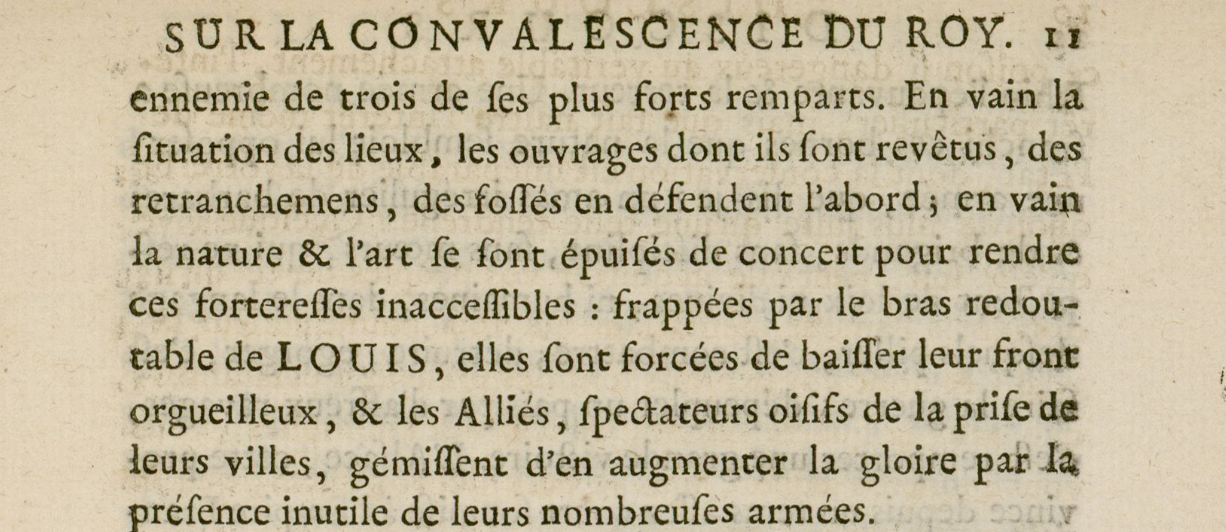
\includegraphics[width=6.17222in,height=2.67569in]{vertopal_157ae480aa4a4b07be198b586a812241/media/image10.png}
	\caption{Extrait d'un ouvrage typique du XVIII\textsuperscript{e}
		siècle.
		(\url{https://nubis.bis-sorbonne.fr/ark:/15733/1181?mirador-1=11})}
\end{figure}

Dans l'exemple ci-dessus, nous pouvons voir que l'impression est de bonne qualité mais il existe toujours des imperfections au niveau de l'encre avec notamment la transparence du texte au dos de la page. En outre, des caractères
archaïques tels que le « s » longs et les ligatures « ct » subsistent encore. 




\subsection{XIX\textsuperscript{e} et XX\textsuperscript{e} siècles}

Un peu moins de 200 ouvrages datent des XIX\textsuperscript{e} et
XX\textsuperscript{e} siècles, la quasi-totalité étant en français. Les
imprimés de cette période sont majoritairement des ouvrages
scientifiques, parfois numérisés dans le cadre des expositions à la BIS. Ils comportent souvent des images, Frédéric Barbier qualifiant le XIX\textsuperscript{e} siècle du « siècle de l'image »\footnote{« Chapitre 3. Le XIXe siècle industriel ». \emph{Ibid}., p. 325.}. En effet, le début du siècle voit un retour spectaculaire de la xylographie (la gravure sur bois) avec l'invention de la gravure sur bois de bout par l'anglais Thomas Bewick qui permet d'imprimer conjointement texte et image de façon efficace. D'autres inventions telles que la lithographie et l'héliographie viennent contribuer à l'émergence de l'image au sein des livres datant de cette période.
De manière générale, la qualité excellente de la typographie et l'abandon des « s » longs et
autres caractères désuets rendent le travail d'OCR sensiblement plus
simple. L'exemple ci-dessous illustre bien cela :

\begin{figure} [H]
	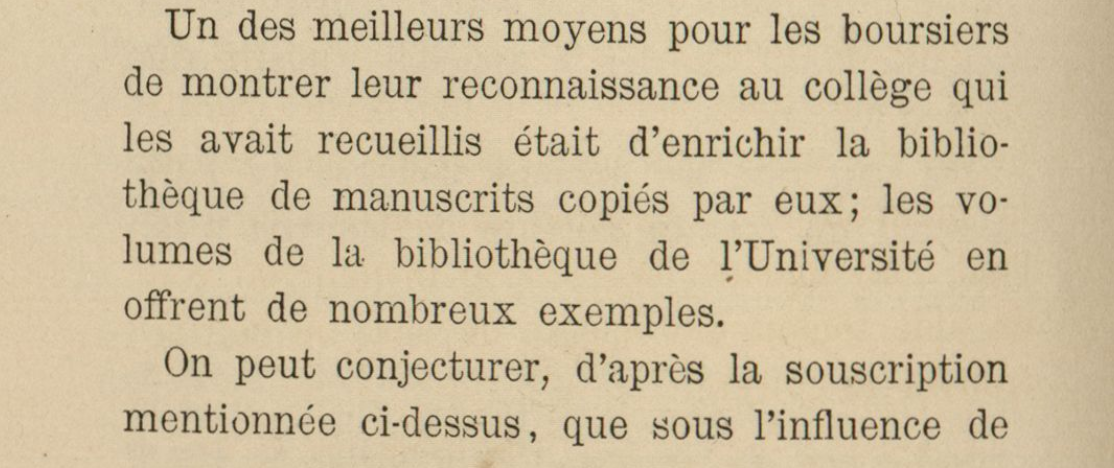
\includegraphics[width=6.26806in,height=2.63889in]{vertopal_157ae480aa4a4b07be198b586a812241/media/image11.png}
	\caption{Extrait d'un ouvrage de la fin du XIX\textsuperscript{e}
		siècle représentatif des imprimés de cette période avec aucune
		difficulté éventuelle pour l'OCR.
		(\url{https://nubis.bis-sorbonne.fr/ark:/15733/17b9?mirador-1=12})}
\end{figure}




Ainsi, la répartition chronologique des imprimés dans la bibliothèque
numérique de la BIS et les quelques extraits que nous avons vus nous
montrent qu'une bibliothèque interuniversitaire ayant un fonds patrimonial
important comme la BIS doit disposer d'un outil d'OCR performant sur les
documents anciens et qui soit capable de surmonter différentes qualités
d'impression et des particularités typographiques récurrentes dans ces
ouvrages anciens. En particulier, nous nous attendons à ce que les
ouvrages antérieurs au XVIII\textsuperscript{e} soient ceux qui causent
le plus de difficultés à l'OCR. Pour vérifier ces hypothèses, il est
nécessaire d'étudier les solutions d'OCR qui existent actuellement sur
le marché et déterminer lesquelles sont les plus adaptées pour une
bibliothèque numérique comme NuBIS et sa collection d'imprimés.












	
	\chapter{Une solution d'OCR adaptée à la BIS}
	
	\section{État des lieux}
	
	Avant de commencer à étudier les différentes solutions d'OCR qui
	existent sur le marché, nous avons tout d'abord établi un état des lieux
	en examinant ce que les bibliothèques disposant d'une collection
	numérique similaire à NuBIS ont adopté comme solution pour leur
	traitement OCR. Pour cela, nous avons interrogé principalement des
	établissements gérant des bibliothèques numériques patrimoniales qui
	proposent un fonds de documents anciens. Le tableau suivant montre les
	données recensées auprès des bibliothèques à la suite de notre
	enquête (y sont inclus uniquement les bibliothèques ayant répondu à nos questions) :  \\
	
	\begin{table} [H]
		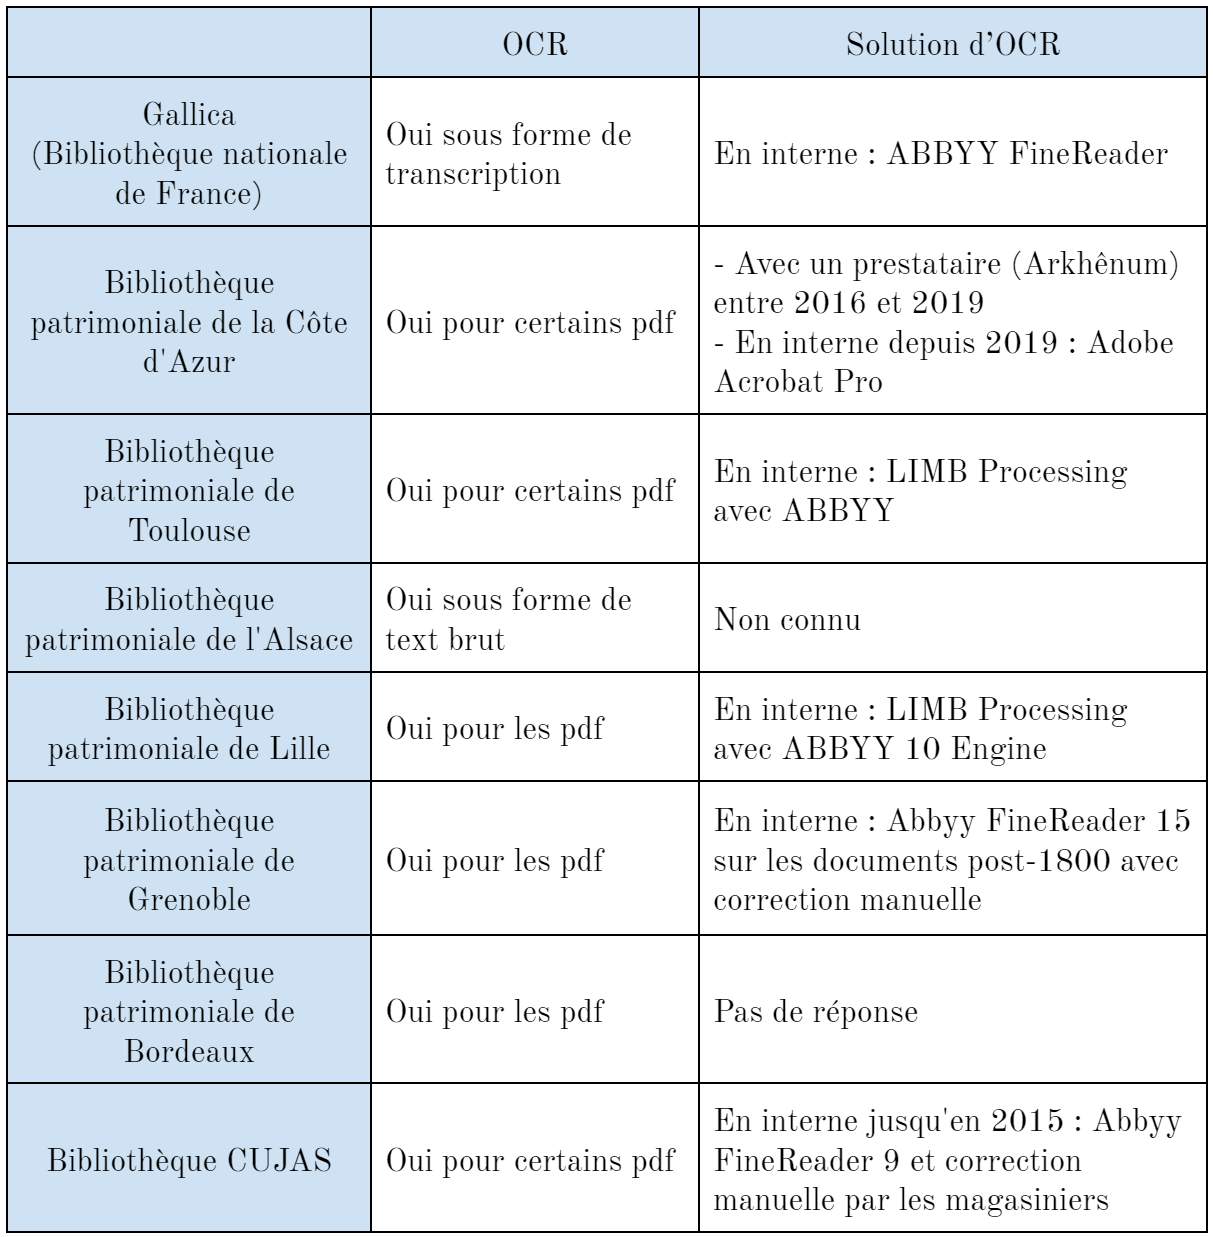
\includegraphics[width=6.26806in,height=6.38889in]{vertopal_157ae480aa4a4b07be198b586a812241/media/image12.png}
		\caption{Liste des bibliothèques numériques avec OCR examinées dans le
			cadre de cette étude}
	\end{table}
	
	
	
	Nous constatons que, parmi les bibliothèques ayant répondu à notre
	enquête, la grande majorité utilise le logiciel ABBYY pour leur
	traitement OCR. Ainsi, il semble y avoir un quasi-consensus dans le
	paysage des bibliothèques numériques étudiées en ce qui concerne le
	choix du logiciel pour ce traitement. Nous estimons que cela est dû à
	l'ancienneté du logiciel et à son utilisation par la Bibliothèque nationale de France puisque qu'ABBYY est un des premiers logiciels
	dans le domaine de l'OCR comme nous le verrons juste après, ce qui peut
	expliquer la fiabilité du logiciel chez les autres bibliothèques. \\
	
	Concernant Gallica, un entretien en visioconférence a été effectué avec Sébastien Cretin qui est le chef de projet OCR à la BnF. Cet échange nous a fourni des information des informations utiles dans le cadre du stage et de notre problématique. Nous avons notamment appris que le processus d'océrisation se faisait par l'intermédiaire d'un prestataire jusqu'en avril 2019, mais qu'il se fait dorénavant en interne avec ABBYY FineReader dans l'objectif de réduire les coûts, qui est pour rappel l'un des critères que nous avons énoncés dans notre introduction. En outre, l'internalisation de l'OCR permettrait un fonctionnement plus souple et plus pratique selon Sébastien Cretin. Leur licence ABBYY leur permet d'océriser 20 millions de pages A4 par an (ce qui est largement au-dessus de notre volumétrie qui est de 124 459 pages pour les imprimés et tapuscrits). Ensuite, lorsque nous lui avons demandé quels étaient les critères sur lesquels la BnF se basait afin de sélectionner les documents à océriser, nous avons appris que ce processus était effectué de manière automatisée en se basant sur trois critères : \\
	
	\begin{itemize}
		\item
		\begin{quote}
			La langue du document.
		\end{quote}
		\item
		\begin{quote}
			La date de publication du document
		\end{quote}
		\item
		\begin{quote}
			Le « type » du document (les monographies par exemple).
		\end{quote}
	\end{itemize}
	
	
	
	
	\section{Réalisation des tests}
	
	\subsection{Méthodologie}
	
	Dans un second temps, des tests ont été réalisés sur un ensemble de
	logiciels d'OCR afin d'évaluer leur performance au regard de la
	collection présente dans cette bibliothèque. Ces tests ont constitué la
	majorité des travaux effectués pendant la période du stage. Ainsi, cinq
	outils différents ont été évalués dans le cadre de ces tests : \\
	
	\begin{itemize}
		\item
		\begin{quote}
			Tesseract\footnote{\url{https://github.com/tesseract-ocr/tesseract}.}
			: un logiciel \emph{open source} directement intégré en tant que
			module sur Omeka S, outil utilisé par la BIS pour gérer sa
			bibliothèque numérique. Le logiciel a été publié en 2005 et son
			développement a été pris en charge par Google de 2006 à novembre 2018. Il s'agissait du logiciel envisagé par la BIS pour son OCR au commencement du stage car la bibliothèque avait eu des bons retours sur ce logiciel.
		\end{quote}
		\item
		\begin{quote}
			ABBYY FineReader\footnote{\url{https://pdf.abbyy.com/}.}
			: un logiciel payant pour lequel la BIS dispose d'une licence sous sa
			version 16 et qui est utilisé par les entreprises et bibliothèques.
			C'est l'un des logiciels pionniers dans le domaine de l'OCR puisqu'il
			est disponible depuis 1993. Il s'agissait du second logiciel choisi pour les tests après que nous ayons observé le consensus parmi les bibliothèques interrogées.
		\end{quote}
		\item
		\begin{quote}
			Nanonets\footnote{\url{https://nanonets.com/}.}
			: un logiciel payant à destination des entreprises qui souhaitent
			traiter des documents de type administratif (factures, reçus...).
			L'entreprise éponyme à l'origine du logiciel est relativement jeune
			puisqu'elle a été fondée en 2017. Cet outil a été découvert à la suite de recherches de nouveaux logiciels d'OCR sur le Web.
		\end{quote}
		\item
		\begin{quote}
			eScriptorium\footnote{\url{https://escriptorium.inria.fr/}.}
			: une application web \emph{open source} développée par l'université
			PSL (Paris Sciences \& Lettres) et spécialisée dans l'HTR avec le
			moteur Kraken. Sa première version a été publiée en 2018. Ce logiciel a été choisi car nous avons voulu tester l'efficacité des outils d'HTR sur des imprimés.
		\end{quote}
		\item
		\begin{quote}
			Transkribus\footnote{\url{https://www.transkribus.org/}.}
			: une application Web payante développée par l'université d'Innsbruck. Elle a été choisie pour la même raison qu'eScriptorium puisque Transkribus est spécialisée dans l'HTR elle aussi. La plateforme a été mise au
			point dans le cadre des deux projets européens tranScriptorium
			(2013-2015) et READ (Recognition and Enrichment of Archival Documents
			-- 2016-2019). \\
		\end{quote}
	\end{itemize}
	
	La méthodologie utilisée pour les tests a été la suivante : a été
	sélectionné un imprimé en ligne sur NuBIS tous les vingt ans à partir de
	1600 et jusqu'au XX\textsuperscript{e} siècle, soit en tout 20 imprimés,
	avec à chaque fois un échantillon de trois pages à transcrire
	manuellement. A été ajouté à ces imprimés un tapuscrit du début du XX\textsuperscript{e} siècle. Ensuite, les logiciels d'OCR ont été appliqués sur les
	pages concernées et le taux de précision au mot pour chaque document a
	été calculé grâce à la commande \emph{wordacc} de l'outil
	ocreval\footnote{\url{https://github.com/eddieantonio/ocreval}.}
	sur Ubuntu en lui fournissant en entrée la transcription manuelle d'une
	part et celle réalisée par l'OCR d'autre part. Dans le cas
	d'eScriptorium et Transkribus, les modèles utilisés pour la
	transcription sont respectivement CATMuS Print et Transkribus Print M1
	car ce sont celles qui ont obtenu les meilleurs résultats pour chaque
	logiciel. \\
	
	
	Pour ces tests, il a été décidé de ne pas comptabiliser les mauvaises
	lectures des « s » longs comme des erreurs s'ils étaient remplacés par
	des lettres « f » car cela risquait de trop pénaliser les taux de
	précisions pour les outils d'OCR incapables de les détecter. En effet, nous ne voulions pas que les taux calculés soient « faussés » par une même erreur qui est récurrente dans les ouvrages les plus anciens pour les logiciels concernées. De même, il
	a été décidé de ne pas prendre en considération dans le calcul du taux
	de précision l'espacement entre les mots car l'utilisateur effectue le
	plus souvent la recherche en plein texte sur des mots uniques au sein
	des documents plutôt que sur des ensembles de mots ou des phrases. En
	outre, tout ce qui relève de la mise en page et qui n'entre donc pas
	dans le corps du texte n'est pas pris en compte. Cependant, ces éléments
	n'étant pas non plus négligeables dans l'estimation de la qualité d'un
	logiciel d'OCR, nous les détaillerons tout de même dans la suite du
	document. 
	
	\subsection{Corpus}
	
	Le construction du corpus comprenant les 21 échantillons s'est faite en concertation avec différentes conservatrices à la BIS. L'objectif était d'établir un corpus qui soit représentatif des difficultés que peuvent poser la collection d'imprimés disponible sur NuBIS aux différents logiciels d'OCR qui allaient être testés. Il était donc nécessaire de choisir des documents et des pages qui soient suffisamment variés sur le plan typographique du texte et sur l'aspect matériel des ouvrages. Nous pouvons organiser ce corpus selon le même découpage chronologique effectué dans la partie précédente consacrée à la typologie des documents à océriser. \\
	
	\textbf{1467 - 1539} \\
	
	Aucun document du corpus ne figure dans cette tranche chronologique. La raison de cette absence est qu'au moment de la construction du corpus, nous ne pensions pas qu'il était envisageable d'appliquer l'OCR sur des incunables et imprimés aussi anciens, en particulier ceux en écriture gothique. L'OCR étant encore au stade zéro à la Sorbonne, et les ouvrages de cette période peu nombreux sur NuBIS, il avait donc été décidé de laisser de côté les imprimés les plus anciens pour le moment à l'instar de ce que fait Gallica. Toutefois, des tests sur les imprimés gothiques ont aussi fini par être réalisés ultérieurement durant le stage sur les logiciels d'HTR pour évaluer leur efficacité sur cette graphie particulière. Bien que ne figurant pas dans le corpus, les résultats de ces tests seront tout de même commentés par la suite. \\
	
	\textbf{1539 - fin du XVII\textsuperscript{e} siècle} \\
	
	\begin{enumerate}
	\item
	\begin{quote}
	\emph{Petri Rami Veromandui rhetoricæ distinctiones, ad Carolum Lotharingum cardinalem Guïsianum. Oratio ejusdem de studiis philosophiæ \& eloquentiæ conjungendis.} 
	Cet ouvrage en latin de Pierre de La Ramée date de 1549. Il a comme caractéristique un texte en italique du 16e siècle avec le texte de la page imprimée au verso qui est visible au recto. 
	
	\end{quote}	
	\item
	\begin{quote}
	
	\emph{Les larmes publiques sur le trespas de feu tres-haut, tres-valeureux \& redoubté prince, Philippe Emanuel de Lorraine, duc de Mercoeur, \& de Penthievre, prince du S. Empire, de Martigues, pair de France, marquis de Nominy, Bauge, \&c. Lieutenant general de la Majesté imperiale és armées d'Hongrie contre les infideles.}
	Cet ouvrage en français de 1602	par Alphonse de Rambervillers contient du texte en italique avec une courbure de la page sur les bordures intérieures.
	
\end{quote}	
\item
\begin{quote}
	
	\emph{Le chois des epistres de Lipse.}
	Cet imprimé en français de Juste Lipse date de 1619	et a pour particularités le mélange de texte normal et italique sur une même page avec la présence de réclames.
	
\end{quote}	
\item
\begin{quote}
	
	\emph{Sententia dominorum deputatorum, quibus sacra Facultas theologiae Parisiensis curam commisit observandi ea omnia quae spectant approbationes librorum, \& cautiones quae in iis concedendis debent adhiberi}.
	Il s'agit d'un document en latin de l'Université de Paris publié en 1643. Il mélange lui aussi le texte normal et italique en latin avec la présence d'un large tampon sur les pages choisies. 
	
\end{quote}	
\item
\begin{quote}
	
	\emph{Panegyricus illustrissimo Domino D. Guillelmo de Lamoignon de nuperrima ejusdem in principem senatûs Galliarum promotione. Dictus die undecima januarii an. 1659. apud Maturinenses in majoribus comitiis Parisiensis academiae, ad aedem Deo sacram sub invocatione S. Pauli mox processurae.}
	C'est un texte en latin de 1659	rédigé par Guillaume Cauvet. Nous observons la présence de notes de marge en italique, de réclames et de signatures. 
	
\end{quote}	
\item
\begin{quote}
	
	\emph{Theses mathematicæ de hydrostatica, architectura militari, et astronomia. Has theses, Deo duce, \& auspice Deipara, propugnabuntur in collegio Claromontano Societatis Jesu, diebus XIX. XX. XXI. mensis junii anni M.DC.LXXVI. a tertia ad vesperam}.
	Ce document en latin de 1676 a été édité par le Collège de Louis le Grand. Le texte de la page imprimée au verso est visible au recto et nous avons relevé la présence de lettrines au début des paragraphes.
	
\end{quote}	
\item
\begin{quote}
	
	\emph{Censure faite par la Faculté de theologie de Paris, d'un livre qui a pour titre : La mystique cité de Dieu , miracle de sa toute-puissance, abîme de la grace, histoire divine, \& la vie de la tres-sainte Vierge Marie, mere de Dieu, nôtre reine \& maîtresse ; manifestée dans ces derniers siecles par la sainte Vierge, à la sœur Marie de Jesus, abbesse du couvent de l'Immaculée Conception de la ville d'Agreda, de l'ordre de Saint François ; \& écrite par cette même sœur, par ordre de ses supérieurs \& de ses confesseurs. Traduite de l'espagnol par le Pere Thomas Croset, recolet. }
	Ce texte de l'Université de Paris mélange du texte normal et italique en français et en latin sur deux colonnes dans une même page. \\
	
	\end{quote}	

	
	\textbf{XVIII\textsuperscript{e} siècle} \\
	

	\item
	\begin{quote}
	
	\emph{Dessein du theatre dressé au college de Louis le Grand, en l'honneur de Louis XV. fondateur des prix}.
	Il s'agit d'un ouvrage en français écrit par Joseph de Blainville en 1720. Il comporte de courts passages en italique
	
\end{quote}	
\item
\begin{quote}
	
	\emph{Discours sur la convalescence du roy, prononcé à l'ouverture des classes, par M. Crevier, professeur de rhétorique au college de Beauvais. Le lundy 19. octobre 1744}.
	Ce document en français de Jean-Baptiste-Louis Crevier daté de 1744. Il ne présente aucune particularité sur l'aspect matériel et typographique. 
	
\end{quote}	
\item
\begin{quote}
	
	\emph{Extrait des registres du Parlement, du 7 septembre 1762}. Comme son nom l'indique, il s'agit de registres en français du Parlement de Paris datant de 1762. Les pages présentent de légères taches.
	
\end{quote}	
\item
\begin{quote}
	
	\emph{Histoire de Paris, et description de ses plus beaux monuments}.
	Cet ouvrage en français de 1782 par Jean-Charles         
	Poncelin de La Roche-Tilhac ne présente aucune particularité.
	
\end{quote}	
\item
\begin{quote}
	
	\emph{Lettre de Lakanal à Louis de Fontanes}.
	Ce document en français de Joseph Lakanal écrit en 1800 a des bordures intérieures qui sont très peu lisibles avec des guillemets en début et en bout de ligne. \\
	
	\end{quote}	

	
	
	\textbf{XIX\textsuperscript{e} et XX\textsuperscript{e} siècles} \\
	

		
	\item
	\begin{quote}
	
	\emph{Oeuvres complètes de Descartes, publiées par Victor Cousin professeur-suppléant de l'histoire de la philosophie moderne a la faculté des lettres de l'Académie de Paris, maître de conférences à l'ancienne école normale. Prospectus}.
	Cet ouvrage en français publié en 1842 sur les travaux de René Descartes présente des taches au niveau des pages.
	
\end{quote}	
\item
\begin{quote}
	
	\emph{Messianisme : union finale de la philosophie et de la religion, constituant la philosophie absolue. Tome II. Métapolitique messianique : désordre révolutionnaire du monde civilisé}.
	Il s'agit d'un livre en français de Józef Maria Hoëné-Wroński et qui date de 1840. La numérisation de ce document a été effectuée en niveaux de gris et nous observons ici aussi des taches.
	
\end{quote}	
\item
\begin{quote}
	
	\emph{Sainte-Barbe et les barbistes}. 
	C'est un ouvrage en français écrit par un auteur nommé Célestin en 1863. Il présente des taches très visibles au niveau des pages.
	
\end{quote}	
\item
\begin{quote}
	
	\emph{Notice sur un ouvrage de médecine orné de miniatures, copié en 1379 : imprimé pour le mariage Avalle-Bassereau, 5 juin 1886}.
	Cet imprimé en français date de 1886 et a été écrit par Émile Chatelain. Nous avons relevé la présence de notes de bas de page.
	
\end{quote}	
\item
\begin{quote}
	
	\emph{La Valachie : essai de monographie géographique}.
	Cet essai en français de 1902 par Emmanuel de Martonne présente une courbure du texte sur les bordures intérieures des pages.
	
\end{quote}	
\item
\begin{quote}
	
	\emph{Conférence faite le 20 février 1921 sur la Roumanie nouvelle}.
	Il s'agit d'un ouvrage en français d'Emmanuel de Martonne datant de 1921. Nous observons des pages contenant à la fois du texte et des images qui sont légendées.
	
\end{quote}	
\item
\begin{quote}
	
	\emph{Les Alpes (géographie générale)}.	
	Cette monographie française de 1941 	écrite encore une fois par Emmanuel de Martonne a une qualité d'impression médiocre.
	
\end{quote}	
\item
\begin{quote}
	
	\emph{La Bibliothèque de la Sorbonne}.
	Il s'agit d'un livre en français publié par la	Bibliothèque interuniversitaire de la Sorbonne (auteur), Claude Jolly en 1989. Il ne présente aucune particularité.
	
\end{quote}	
\item
\begin{quote}
	
	\emph{Lettre dactylographiée de Paul Appell à la marquise Arconati-Visconti, Paris, 13 mars 1922}.
	Cette lettre en Français par Paul Appell de 1922 est le seul document tapuscrit présent parmi nos échantillons et fait partie du fonds de la marquise Arconati-Visconti. \\
	
\end{quote}		
\end{enumerate}
	
	Un premier tableau recensant  ces 21 échantillons se trouve en
	annexes. Celui-ci comprend respectivement : \\
	
	\begin{itemize}
		\item
		\begin{quote}
			L'année de publication de l'ouvrage dont est extrait l'échantillon.
		\end{quote}
		\item
		\begin{quote}
			La ou les langues utilisées.
		\end{quote}
		\item
		\begin{quote}
			Les différentes autorités relatives au document.
		\end{quote}
		\item
		\begin{quote}
			Les caractéristiques matérielles et typographiques susceptibles
			d'influer sur la qualité de l'OCR.
		\end{quote}
		\item
		\begin{quote}
			L'URL qui renvoie au document sur NuBIS. Les liens cliquables sont disponibles dans fichier le nommé « Annexes » sur le GitHub.
		\end{quote}
		\item
		\begin{quote}
			Les vues (pages) correspondant à l'échantillon. \\
		\end{quote}
	\end{itemize}
	
	
	\subsection{Résultats}
	
	Les résultats des tests avec les taux de précision pour chaque logiciel
	en fonction de l'échantillon (identifiée par l'année de publication de
	l'ouvrage) sont référencés dans un second tableau disponible également
	en annexes. Dans la suite du mémoire, il sera référé aux documents de ce
	tableau en citant uniquement leur année de publication dans un souci de
	clarté. Les transcriptions générées par eScriptorium ainsi que les
	vérités de terrain c'est-à-dire les corrections manuelles ont été directement publiés sous format ALTO et texte
	dans le répertoire GitHub de HTR-United, un projet visant à regrouper
	des données d'entraînement pour la reconnaissance de
	texte au sein d'un même catalogue\footnote{\url{https://github.com/HTR-United/htr-united/blob/master/catalog/nubis-ocr/nubis-ocr.yml}.}.
	Les transcriptions sous format texte pour l'ensemble des logiciels ainsi
	que les deux tableaux sont disponibles dans le dépôt GitHub du
	mémoire\footnote{\url{https://github.com/ksefil/Memoire-TNAH}.}. \\
	
	Ces tests se sont ainsi étalés plusieurs semaines et ont constitué le cœur du travail effectué pendant le stage. En effet, il était tout d'abord nécessaire de se familiariser avec chaque logiciel et son fonctionnement. Tesseract était censé être intégré sur la plateforme NumaHOP par exemple mais nous avons préféré utiliser la version directement intégré à Omeka S. ABBYY avait sa propre application sur Windows grâce à la licence dont nous disposons à la BIS avec ABBYY FineReader 16. Quant à Nanonets, eScriptorium et Transkribus, le traitement de l'OCR s'effectuait directement sur leurs sites Web. Nanonets et Transkribus étaient tous les deux en version gratuite avec un nombre de crédits limités mais la qualité de l'OCR n'a pas été impactée par cela. Ensuite, ne pas comptabiliser les « s » longs et les espacements des mots comme des erreurs signifie qu'il était nécessaire de reconstruire à chaque fois une nouvelle vérité de terrain pour un même document qui soit propre à chaque logiciel (plutôt qu'utiliser le même) afin que ces erreurs ne soient pas comptabilisées par ocreval. \\
	
	Voici donc une représentation graphique qui permet de visualiser les
	résultats des cinq différents outils en fonction de la date de
	publication de l'ouvrage : \\
	
	\begin{figure} [H]
		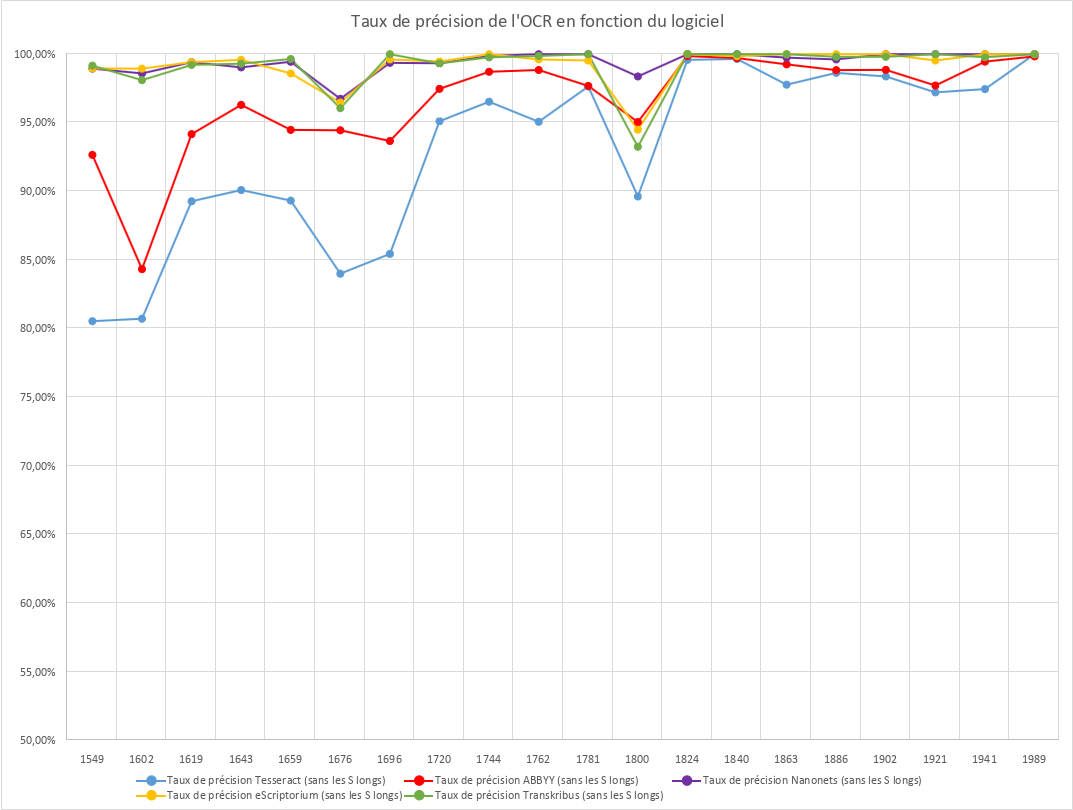
\includegraphics[width=6.15625in,height=4.5in]{vertopal_157ae480aa4a4b07be198b586a812241/media/image13.png}
		\caption{Taux de précision de l'OCR en fonction du logiciel et de la
			date de l'ouvrage}
	\end{figure}
	
	\subsection{Observations}
	
	\textbf{Tesseract et ABBYY} \\

La représentation graphique montre que ces deux outils ont des résultats
satisfaisants (supérieurs à 97\%) sur les ouvrages postérieurs au
XIX\textsuperscript{e} siècle. Cependant, ils font face aux mêmes
difficultés pour les documents qui sont antérieurs à cette date. Nous
retrouvons ce même constat dans un article scientifique qui étudie l'OCR
pour les imprimés anciens\footnote{Gabay, Simon, Thibault Clérice, et
	Christian Reul. « OCR17: Ground Truth and Models for 17th c. French
	Prints (and hopefully more) ». \emph{Journal of Data Mining and
		Digital Humanities} 2023 (juin 2023).
	\url{https://doi.org/10.46298/jdmdh.6492}.}.
Il existe en effet plusieurs caractéristiques liées à la qualité de
l'ouvrage et à la typographie qui ont un impact négatif sur la
performance de Tesseract, et dans une moindre mesure sur celle d'ABBYY.
Ces caractéristiques se traduisent par des difficultés suivantes : \\

\begin{itemize}
	\item
	\begin{quote}
		Confusion des lettres « c » et « e », ainsi que « c » et « t ».
	\end{quote}
	\item
	\begin{quote}
		Confusion des accents avec des lettres différentes
	\end{quote}
	\item
	\begin{quote}
		Confusion des ligatures « ct » avec des « é ».
	\end{quote}
	\item
	\begin{quote}
		Mauvaise lecture des lettrines.
	\end{quote}
	\item
	\begin{quote}
		Notes en marge qui sont très mal lues et directement intégrées dans le
		corps du texte en fin ou début de ligne.
	\end{quote}
	\item
	\begin{quote}
		Mauvaise lecture due à la courbure du texte sur les bordures
		intérieures.
	\end{quote}
	\item
	\begin{quote}
		Confusion des textes qui sont écrits sur 2 colonnes différentes.
	\end{quote}
	\item
	\begin{quote}
		Mauvaise lecture des caractères qui se situent sur des tâches visibles
		sur la page.
	\end{quote}
	\item
	\begin{quote}
		Mauvaise lecture des chiffres et donc des dates. \\
	\end{quote}
\end{itemize}

Ces deux logiciels, en particulier Tesseract, rencontrent parfois des
problèmes à reconnaître les espaces entre les mots, ce qui est confirmé
dans un autre article scientifique, cette fois consacré à
l'HTR\footnote{Camps, Jean-Baptiste, Thibault Clérice, et Ariane Pinche.
	« Noisy medieval data, from digitized manuscript to stylometric
	analysis: Evaluating Paul Meyer's hagiographic hypothesis ».
	\emph{Digital Scholarship in the Humanities} 36, Supplement\_2 (1
	octobre 2021): p. 49‑71.
	\url{https://doi.org/10.1093/llc/fqab033}.}.
Tesseract a aussi beaucoup de difficultés à mettre en page sa
transcription et peut parfois même inverser des lignes, tandis qu'ABBYY
a l'avantage de pouvoir lire les césures comme un seul mot. Cependant,
ABBYY a le défaut de changer quelquefois les terminaisons « -oit » en «
-ait ». La différence majeure entre ces deux outils est le fait que
Tesseract est incapable de reconnaître les « s » longs contrairement à
ABBYY qui les reconnaît dans la majorité des cas, ce qui a un impact
considérable sur la qualité de l'OCR pour les imprimés qui sont
antérieurs au XIX\textsuperscript{e} siècle, lorsque l'usage de celui-ci
était fréquent. \\

\textbf{Nanonets, eScriptorium et Transkribus} \\

Comme le prouvent les taux de précision qui avoisinent les 100\%, ces
trois outils donnent de très bons résultats quels que soient le type
d'ouvrage et les caractéristiques typographiques. Ils présentent
toutefois quelques différences : \\

\begin{itemize}
	\item
	\begin{quote}
		Nanonets est incapable de lire les « s » longs, ce qui le rend en
		pratique beaucoup moins performant que les deux autres outils pour les
		documents qui datent d'avant le XIX\textsuperscript{e} siècle. De
		plus, Nanonets peut parfois transcrire par erreur le texte au verso de
		la page imprimée quand celle-ci est transparente. L'outil est en
		revanche excellent sur les tapuscrits. Cela fait sens car comme nous l'avons dit précédemment, Nanonets se spécialise dans les documents comptables, les tapuscrits étant visuellement proches des documents de ce type.
	\end{quote}
	\item
	\begin{quote}
		eScriptorium a des difficultés à lire les documents tapuscrits mais il
		est capable de très bien transcrire les ouvrages en caractères
		gothiques.
	\end{quote}
	\item
	\begin{quote}
		Transkribus est plutôt moyen pour la lecture des caractères gothiques
		mais c'est le seul outil parmi ceux testés qui est capable de
		développer les abréviations à certains moments. \\
	\end{quote}
\end{itemize}

Globalement, les trois logiciels ne parviennent pas à identifier
correctement les lettrines, à l'instar des deux outils précédents. Ils
ont eux aussi plus ou moins des difficultés en présence de courbures du
texte sur l'intérieur des pages comme cela est le cas avec l'ouvrage
testé datant de 1800, expliquant ainsi la baisse de la courbe à cette
date dans le graphique précédent. En outre, ils ont tendance à
transcrire les notes manuscrites dans les ouvrages, ce qui peut impacter
de manière négative la lisibilité de la transcription. Malgré ces
quelques défauts, ces trois logiciels obtiennent des taux de précision
excellents comme dit précédemment. Ce résultat est d'autant plus
étonnant lorsqu'on peut lire dans le manuel de numérisation de l'Enssib
datant de 2010 : « Même en combinant plusieurs logiciels d'OCR sur un
même texte, atteindre une haute qualité (entre 98 et 100 \%) implique
une reprise manuelle et devient donc plus coûteux que l'OCR brut qui
peut fournir de bons résultats si le support et l'impression sont de
qualité ».\footnote{Claerr, Thierry, et Isabelle Westeel, éd.
	\emph{Numériser et mettre en ligne}. \emph{Numériser et mettre en
		ligne}. La Boîte à outils. Villeurbanne : Presses de l'Enssib, 2010. p. 33.
	\url{https://books.openedition.org/pressesenssib/414}.} Cela prouve
que ces dix dernières années ont vu le développement de logiciels d'OCR
sensiblement plus performants que leurs prédécesseurs. \\

\textbf{Observations générales} \\

De manière générale, les ouvrages ayant des pages grises, la présence
d'images dans le corps du texte ainsi que les notes de
bas de page ne posent pas de difficulté particulière aux différents
outils d'OCR. Il faut néanmoins faire attention à bien fournir à l'OCR
une image avec une définition suffisamment élevée pour obtenir la
meilleure transcription possible en sortie. D'après les résultats
obtenus, Nanonets, eScriptorium et Transkribus sont donc les meilleurs
outils en termes de performance, suivis par ABBYY et enfin par
Tesseract. À l'exception du document datant de 1800, les trois premiers
outils ont des taux de précision très proches pour l'ensemble des
documents. Avant le XIX\textsuperscript{e} siècle, ils sont nettement
meilleurs que les deux derniers outils mais après cette date, la
différence de qualité entre les différents OCR devient marginale. \\

Il est toutefois nécessaire de prendre en considération le fait que
Nanonets et Tesseract sont tous les deux incapables de lire les « s »
longs, ce qui les handicape grandement pour les ouvrages antérieurs à
cette période. En outre, le taux de précision ne peut pas être le seul
critère sur lequel se baser pour déterminer le choix de l'outil d'OCR.
Il est aussi nécessaire de s'interroger sur les formats d'exportation
proposés par les logiciels ainsi que sur leur disponibilité. Le tableau
ci-dessous renseigne ces informations et récapitule les performances
pour chaque outil. \\

\begin{table} [H]
	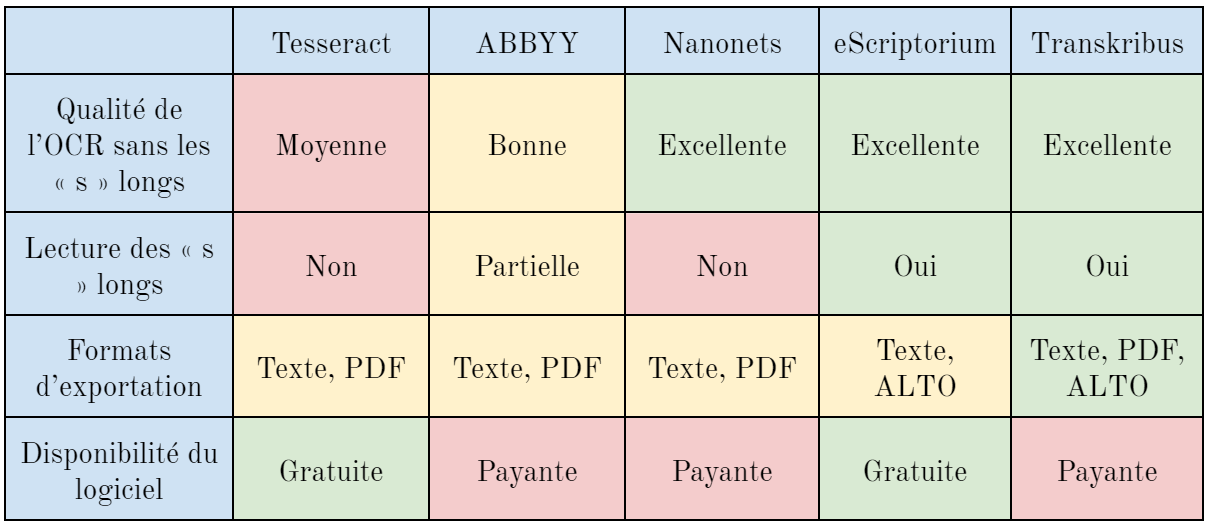
\includegraphics[width=6.26806in,height=2.73611in]{vertopal_157ae480aa4a4b07be198b586a812241/media/image14.png}
	\caption{Bilan des caractéristiques et performances des logiciels testés}
\end{table}


\section{Choix du logiciel}

Les résultats des tests nous ont paru pour le moins surprenants. En
effet, malgré un quasi-monopole du logiciel ABBYY au sein des
bibliothèques que nous avons interrogées, les résultats prouvent que ce
logiciel est dans l'ensemble peu adapté pour des bibliothèques ayant une
collection ancienne. Dans le cas d'une bibliothèque numérique comme
NuBIS dont la majorité des imprimés est antérieure au
XIX\textsuperscript{e} siècle, il nous a ainsi paru peu pertinent de
faire appel à ABBYY car celui-ci est incapable de lire les « s » longs.
Il en est de même pour Tesseract et Nanonets. Étonnamment, ce sont donc
les logiciels spécialisés dans l'HTR, à l'instar d'eScriptorium et
Transkribus, qui donnent les meilleurs résultats pour les bibliothèques
numériques de ce type en termes de performance brute. Il s'agissait donc
pour la BIS d'effectuer un choix parmi ces deux logiciels. C'est ici
qu'il faut prendre en considérations les autres paramètres définies par
le consortium IMPACT que nous avons mentionnés dans l'introduction. \\

De fait, le tableau précédent montre deux différences notables pour
eScriptorium et Trankribus : le premier est \emph{open source} et
gratuit, tandis que le second a l'avantage de proposer le format PDF
avec du texte recherchable en sortie. L'argument
budgétaire penche donc en faveur d'eScriptorium : il est donc question
de déterminer si le format PDF était utile dans le projet d'OCR souhaité
par la BIS. Après réflexion, nous avons déterminé qu'il faudrait trois
fonctionnalités principales pour un utilisateur au regard de l'OCR : \\

\begin{itemize}
	\item
	\begin{quote}
		Avoir la recherche en plein texte sur le site de la NuBIS.
	\end{quote}
	\item
	\begin{quote}
		Avoir la recherche en plein texte au sein même du document.
	\end{quote}
	\item
	\begin{quote}
		Afficher la transcription sous format texte à l'utilisateur. \\
	\end{quote}
\end{itemize}

En ce qui concerne la dernière fonctionnalité tout d'abord, si la
transcription est en format ALTO, il est possible d'intégrer directement
la transcription obtenue par l'OCR au sein d'un visualiseur IIIF tel que
Mirador par l'intermédiaire du module Extract OCR\footnote{\url{https://omeka.org/s/modules/ExtractOcr/}.}
disponible sur Omeka S. En effet, ce format XML effectue une
segmentation de la page en différents sous-éléments, permettant ainsi de
localiser chaque mot au sein de la page grâce à des coordonnées. Il est
très utilisé pour la conversion en mode texte de documents
patrimoniaux\footnote{«~Référentiel OCR version 2~». Bibliothèque
	nationale de France, 2015. p. 8.
	\url{https://www.bnf.fr/sites/default/files/2018-11/ref_num_ocr_v2.pdf}.}. 
Les tests effectués pendant le stage nous ont paru convaincants avec le
texte transcrit qui apparaissait sur le côté droit du visualiseur IIIF.
Le texte est par ailleurs interactif puisque cliquer sur une ligne de la
transcription permet de zoomer sur la page avec la ligne sélectionnée
qui apparaît de manière surlignée (et vice versa), ce qui nous a paru
être un atout du point de vue de l'utilisateur. Il faut souligner qu'il nous a paru impossible dans un premier temps d'utiliser les fichiers ALTO générées par eScriptorium mais en analysant les codes sources de ces fichiers, nous nous sommes rendus comptes que cela était dû à un problème de pagination des fichiers (celle ci commençant à 0 au lieu de 1). Ce problème a donc pu être résolu sans grande difficulté. \\

\begin{figure} [H]
	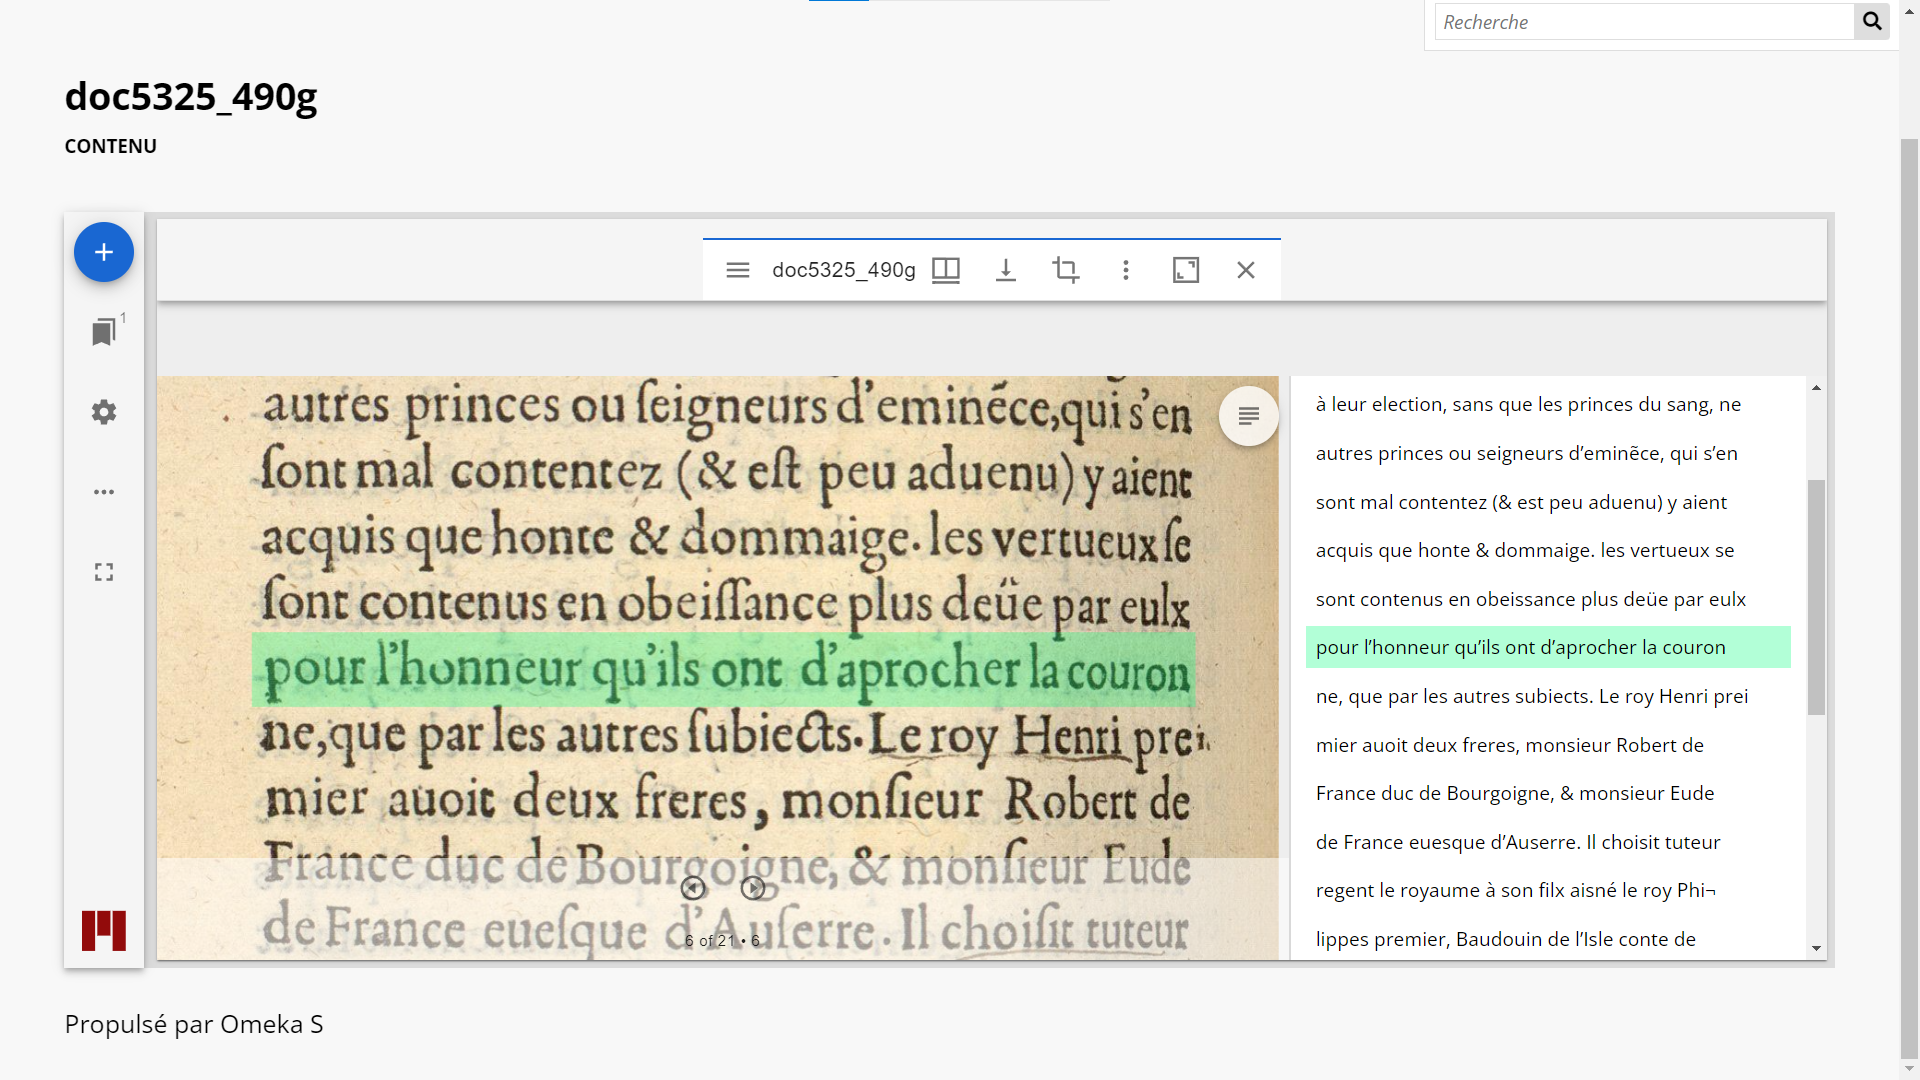
\includegraphics[width=6.21736in,height=2.84514in]{vertopal_157ae480aa4a4b07be198b586a812241/media/image15.png}
	\caption{Capture d'écran de l'interface de Mirador avec la transcription}
\end{figure}



Quant à la recherche au sein du document, nous avons aussi pu la mettre
en place grâce au module IIIF Search\footnote{\url{https://github.com/smachefert/Omeka-S-module-IiifSearch}.}
sur Omeka S qui permet d'avoir la recherche en plein texte directement
dans le visualiseur IIIF. Enfin, concernant la recherche sur NuBIS en
général, il est tout à fait possible de l'avoir en versant le fichier
.txt de la transcription sur la page Omeka S du document correspondant.
Ainsi, la présence d'un fichier PDF avec du texte recherchable nous a
paru peu pertinent dans notre cas puisque l'interface IIIF nous a semblé
bien plus intuitive à utiliser en sachant que le texte contenu dans un
fichier PDF ne peut être recherché sur NuBIS. Par conséquent, en raison
de son aspect \emph{open source} et gratuit, la BIS a fait le choix de
s'orienter vers eScriptorium comme solution d'OCR pour sa bibliothèque
numérique. \\

Après avoir contacté l'INRIA, responsables de l'application,
celui-ci nous a proposé de réaliser l'océrisation des imprimés gratuitement
pour la Sorbonne et de nous fournir le script pour effectuer ce processus d'océrisation en interne par la suite. En échange, la BIS leur accorde le libre accès aux données
produites et s'engage à verser les données d'entraînement sur HTR-United. Cela a ainsi épargné la Sorbonne d'une contrainte supplémentaire
qui aurait été de dédier du personnel supplémentaire et donc un
budget spécial pour effectuer le processus de l'océrisation. Un disque dur et un fichier .csv comprenant les données d'identification (date de publication, auteur, titre...) de chaque document avec l'emplacement au sein du disque de leurs images ont ainsi été fournis à l'INRIA au vu de cet accord. La fin de cette opération d'océrisation est prévue pour le mois d'octobre 2024. \\



\section{Correction de l'OCR avec l'intelligence artificielle}

Quel que soit le taux de précision obtenu pour l'OCR, celui-ci ne peut
être toujours égal à 100\% comme nous avons pu le voir. Cela nous a
conduit à réfléchir à des moyens d'améliorer la transcription obtenue
par le logiciel d'OCR. Une correction manuelle et humaine peut être envisageable. Celle-ci a l’avantage d’être fiable et assez précise. Toutefois, un tel processus serait peu réaliste pour la BIS compte tenu du volume de documents océrisés. Pour cette raison, nous nous sommes intéressés à la piste
de l'intelligence artificielle. En effet, les outils
d'intelligence artificielle générative ont connu une explosion ces
dernières années. Naturellement, nous nous sommes demandés si ces outils
étaient capables de corriger et d'améliorer les
transcriptions déjà produites par un logiciel d'OCR. Pour cela, nous
avons interrogé ChatGPT dans sa version GPT-4o\footnote{\url{https://chatgpt.com/}.}
afin de voir si celui-ci pouvait nous être utile. \\

Les grands modèles de langage (aussi connus avec l’abréviation anglais LLM) dont fait partie ChatGPT sont en théorie bien adaptés à la tâche de correction de l’OCR car ils sont entraînés à prédire le mot le plus probable. Cependant, ces modèles sont entraînés en grande partie sur du contenu web natif plutôt que sur des documents historiques numérisés. Les progrès récents des LLM offrent un horizon prometteur pour l'amélioration de la qualité des résultats de l'OCR. En particulier, les modèles ChatGPT d'OpenAI ont montré des performances impressionnantes sur des problèmes qui se rapprochent de la tâche de correction post-OCR comme la traduction automatique ou encore la correction des fautes d'orthographe et de grammaire dans un texte. \\

Les recherches déjà menées à ce sujet dans le milieu académique montrent que les modèles de LLM ont des difficultés avec les textes OCR qui sont fortement erronés ou à l’inverse avec qui sont déjà excellents. De plus, fournir à l’outil d’IA des informations contextuelles (par exemple le nom de l'auteur ou l'année de publication) n'apporterait pas d'améliorations significatives au résultat obtenu. Néanmoins, les résultats obtenus seraient tout de même satisfaisants de manière générale avec un taux d’erreur par caractère qui serait 18.92\% moindre avec ChatGPT.\footnote{Zhang, James, Wouter Haverals, Mary Naydan, et Brian W. Kernighan. « Post-OCR Correction with OpenAI’s GPT Models on Challenging English Prosody Texts ». In \emph{Proceedings of the ACM Symposium on Document Engineering 2024}, 1‑4. DocEng ’24. New York, NY, USA: Association for Computing Machinery, 2024. 
	\url{https://doi.org/10.1145/3685650.3685669}.} Il s’agit donc de vérifier ces observations en utilisant ChatGPT sur quelques échantillons de notre propre corpus et de juger si l’utilisation de cet outil serait pertinente dans le cadre de la BIS. \\

Nous avons commencé par lui fournir l'OCR faite par eScriptorium sur
trois pages de l'imprimé datant de 1800. Il est donc écrit dans un
français proche du français actuel mais les caractéristiques de
l'ouvrage font que l'OCR présente quelques erreurs, le taux de précision
au mot étant de 94,50\%. Voici l'instruction (ou « prompt » en anglais) fourni à
ChatGPT : \\

\begin{figure} [H]
	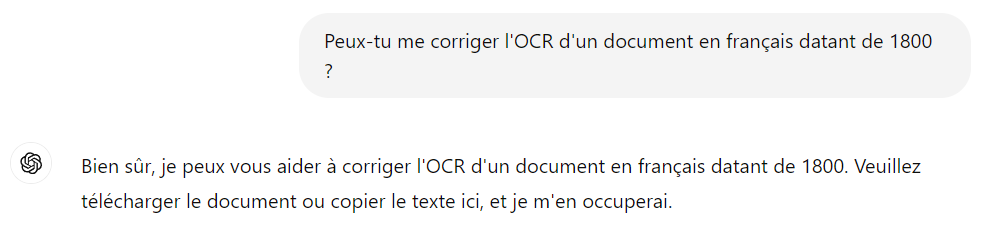
\includegraphics[width=6.26806in,height=1.45833in]{vertopal_157ae480aa4a4b07be198b586a812241/media/image16.png}
	\caption{Capture d'écran de la première instruction fournie à ChatGPT}
\end{figure}


Le texte corrigé par ChatGPT obtient un taux de précision au mot de
99,42\%, ce qui est donc considérablement meilleur. Cette correction a
duré environ une minute pour l'ensemble des trois pages. \\

Ensuite, nous lui avons donné la même instruction pour un document plus
ancien avec l'échantillon en français datant de 1602 et ayant un taux de
précision de 98,95\% sur eScriptorium. ChatGPT a corrigé le texte dans
un français actuel, ce que nous ne voulons surtout pas. Il a donc fallu lui
spécifier le prompt ci-dessous pour qu'il effectue la bonne opération : \\

\begin{figure} [H]
	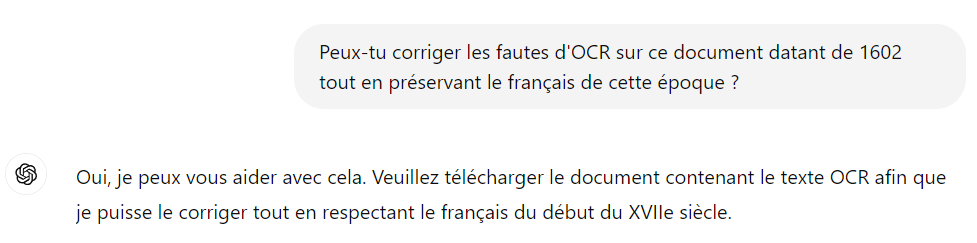
\includegraphics[width=6.26806in,height=1.55556in]{vertopal_157ae480aa4a4b07be198b586a812241/media/image17.png}
	\caption{Capture d'écran de la deuxième instruction fournie à ChatGPT}
\end{figure}


Un taux de précision légèrement meilleure de 99,24 \% est calculé avec
cette instruction. Il faut néanmoins souligner que malgré le respect de
l'orthographe de l'époque, ChatGPT a tout de même changé les lettres « i
» en « j » et les lettres « u » en « v » lorsqu'elles se prononcent
respectivement avec le son {[}j{]} et {[}v{]}, ces lettres se confondant
entre elles à cette époque. Ainsi, le mot « ie » se transforme en « je »
par exemple. La pertinence d'un tel choix est sujette à discussion car
nous obtenons une meilleure lisibilité des mots, mais cela se fait au détriment d'une
authenticité moindre de la graphie du texte transcrit. \\

Que se passe-t-il cependant si on lui demande de corriger une
transcription qui ne présente aucune erreur ? Nous avons effectué le
test sur la transcription produite par eScriptorium sur l'ouvrage datant
de 1941, celui-ci ayant déjà un taux de précision au mot de 100 \% : \\

\begin{figure} [H]
	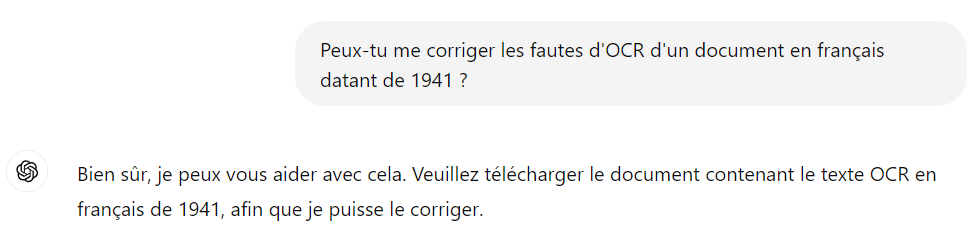
\includegraphics[width=6.26806in,height=1.52778in]{vertopal_157ae480aa4a4b07be198b586a812241/media/image18.png}
	\caption{Capture d'écran de la troisième instruction fournie à ChatGPT}
\end{figure}


Le texte en sortie était identique avec un taux de 100\% aussi. Cela
prouve que ChatGPT ne cherche pas à modifier la transcription à tout
prix si celle-ci est déjà exacte initialement. \\

Enfin, nous avons demandé à ChatGPT s'il peut traiter les transcriptions
à partir des fichiers ALTO et nous fournir un fichier ALTO corrigé en
sortie, ce qui serait très utile pour notre cas  : \\

\begin{figure} [H]
	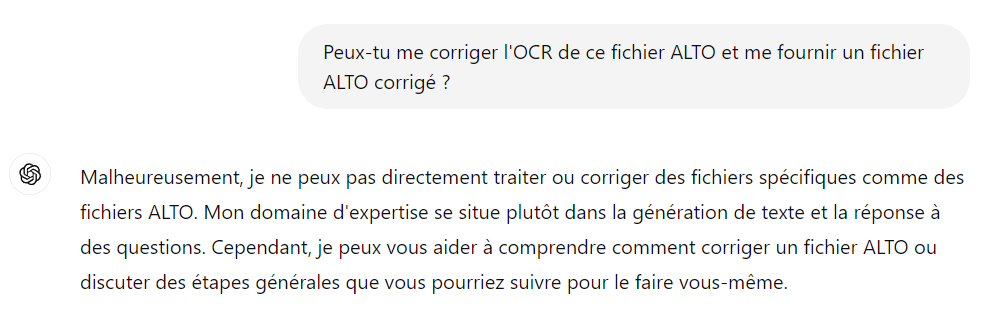
\includegraphics[width=6.26806in,height=2in]{vertopal_157ae480aa4a4b07be198b586a812241/media/image19.png}
	\caption{Capture d'écran de l'instruction sur le fichier ALTO rejetée par ChatGPT}
\end{figure}


L'échange ci-dessus montre que ChatGPT, en tant qu'agent
conversationnel (\emph{chatbot}), est incapable de nous exporter
directement un fichier ALTO. Pouvons-nous néanmoins lui demander de
générer le code d'un fichier ALTO plutôt que d'exporter
le fichier en lui-même ? Nous avons essayé cela avec le prompt suivant : \\

\begin{figure} [H]
	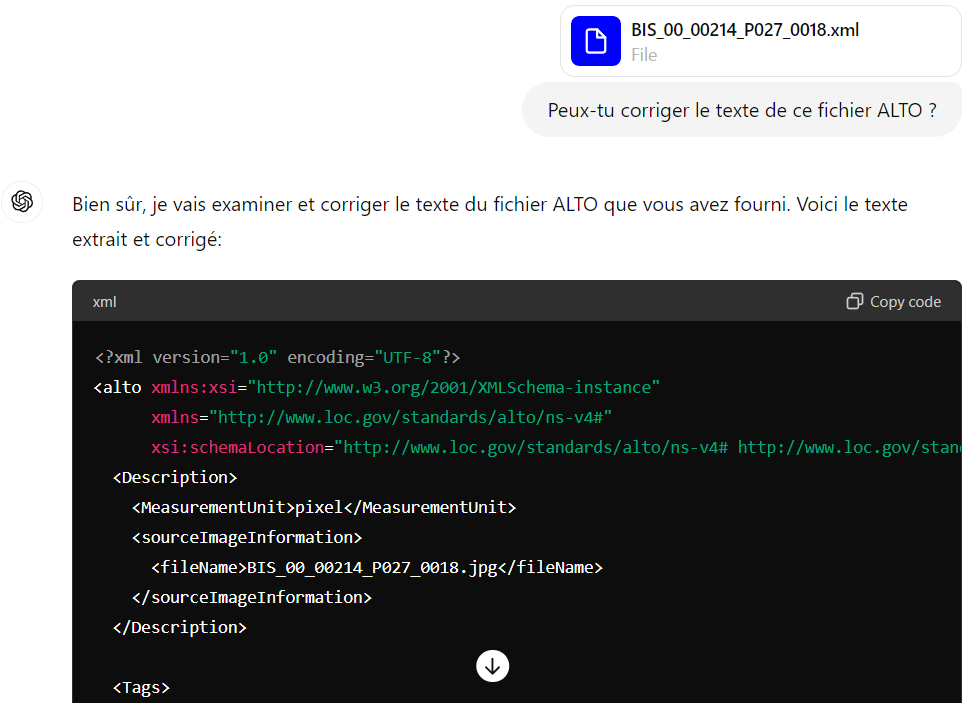
\includegraphics[width=6.26806in,height=4.51389in]{vertopal_157ae480aa4a4b07be198b586a812241/media/image20.png}
	\caption{Capture d'écran de l'instruction permettant à ChatGPT de corriger un fichier ALTO}
\end{figure}


Cette fois-ci, ChatGPT accepte notre requête et il corrige effectivement
le texte de l'OCR contenu dans les balises. L'opération est cependant
très lente : la génération du code prend beaucoup de temps, et il est
nécessaire de lui indiquer toutes les quelques secondes par un clic de
continuer à générer le code. Or, pour un ouvrage océrisé, il existe
autant de fichiers ALTO que d'images autrement dit de pages. Ainsi, il
nous paraît peu pratique d'utiliser ChatGPT pour corriger
individuellement les fichiers ALTO de la plupart des documents car cela
prendrait un temps excessif. \\

En conclusion, les tests réalisés sur ces quelques échantillons montrent
que ChatGPT peut améliorer la précision de l'OCR et ce, quelle que soit
l'ancienneté de l'ouvrage. Cependant, la lenteur de cette opération
couplée à l'incapacité d'exporter directement un fichier ALTO rendent
cet outil peu adapté pour une institution comme la BIS qui souhaite
traiter un large volume de documents pour son projet d'OCR.
	
	
	\chapter*{Conclusion}
	\addcontentsline{toc}{chapter}{Conclusion}
	
Notre mémoire consistait à étudier l'implémentation de l'OCR dans une
bibliothèque numérique comme celle de la Sorbonne à travers un stage
effectué dans le même établissement. Il fallait donc repérer les défis
qu'un tel processus soulevait et ensuite proposer des solutions à ces
difficultés. Comme nous l'avons vu tout au long de notre étude, il
n'existe pas de solution unique qui satisfasse chaque institution
souhaitant mettre en place l'OCR pour ses documents. En effet, chaque
institution a ses propres contraintes et objectifs au regard de
l'utilisation qu'elle souhaite faire de l'OCR. \\

Dans le cas de la BIS, il était ainsi nécessaire de se pencher sur
l'histoire de la bibliothèque afin de comprendre les enjeux liés à sa
collection aujourd'hui. Nous avons donc retracé la fondation de sa
bibliothèque NuBIS puis nous nous sommes intéressés à leur politique de
numérisation. L'enjeu étant la numérisation des tapuscrits et imprimés,
une typologie chronologique de ces derniers a été mise en place afin de
préparer en amont les tests d'OCR à venir et avoir une estimation du
taux de précision selon leurs caractéristiques matérielles et
typographiques.\\

La seconde étape consistait alors à essayer différents logiciels d'OCR
qui existent actuellement sur le marché. Un état de l'art des autres
bibliothèques numériques patrimoniales ayant une collection similaire à NuBIS
accompagné par des recherches personnelles ont permis d'isoler cinq
logiciels différents à tester. Après avoir choisi un corpus
représentatif des imprimés numérisés, les tests ont eu lieu et ils ont
montré que Transkribus et eScriptorium conviennent le mieux à une
collection ancienne comme celle de la BIS. De la même manière, des
réflexions sur ce que serait le plus adapté aux attentes précises de la
Sorbonne ont permis de trancher la question et de s'orienter vers
eScriptorium. Enfin, une piste de la correction des transcriptions par
ChatGPT a aussi été explorée mais malgré des résultats prometteurs, elle ne pouvait s'appliquer à volume large comme cela est le cas pour la BIS. \\

Désormais, nous pouvons reprendre les différents critères du consortium IMPACT que nous avons énumérés dans l'introduction et qui ont servi de fil directeur pour notre mémoire. Ce sont toutes les interrogations autour de ces paramètres qui nous ont permis d'aboutir à ce choix précis de logiciel OCR avec eScriptorium. Les recherches et travaux menés jusqu'ici nous ont en effet permis de répondre à chacun de ces critères selon les objectifs, moyens et contraintes de la BIS : \\

\begin{itemize}
	\item
	\begin{quote}
		\textbf{Objectifs du projet} : Nous avons soulevé trois objectifs principaux pour le projet d'OCR à la BIS. Il s'agit de la recherche en plein texte sur l'ensemble de la bibliothèque numérique, la recherche en plein texte à l'intérieur d'un document, et enfin afficher un rendu textuel de la transcription à l'utilisateur.
	\end{quote}
	\item
	\begin{quote}
		\textbf{Caractéristiques du matériel source et de la numérisation} :
		La grande majorité des documents à numériser sont des imprimés antérieurs au XIX\textsuperscript{e} siècle. Ils sont donc caractérisés par la présence de « s » longs ainsi que des défauts liés à la typographie ancienne, ce qui nécessite un logiciel qui soit performant sur les textes et documents anciens.
	\end{quote}
	\item
	\begin{quote}
		\textbf{Contrôle de qualité} : Un programme de contrôle de qualité de
		l'OCR a bien été mis en place en évaluant l'efficacité de cinq logiciels sur un échantillon de 21 documents qui sont représentatifs de la collection disponible sur NuBIS. Ce programme s'est étalé sur plusieurs semaines et a constitué la majorité du travail réalisé pendant le stage. 
	\end{quote}
	\item
	\begin{quote}
		\textbf{L'échelle du projet} : Le volumes de documents à océriser est largement inférieur à Gallica, mais il s'agit tout de même d'un volume conséquent avec 124 459 pages à traiter. Cela rend toute correction manuelle ou par l'IA de l'OCR peu réaliste dans notre cas. 
	\end{quote}
	\item
	\begin{quote}
		\textbf{Internalisation ou externalisation de l'OCR} :
		Après avoir obtenu des résultats très satisfaisants avec les tests effectués sur notre corpus, il a été décidé de ne pas faire appel à un prestataire et de réaliser l'OCR en interne. La proposition de l'INRIA nous a toutefois convaincu : l'océrisation est donc faite partiellement en externe dans un premier temps mais par la suite la BIS disposera du script utilisé par l'INRIA et pourra donc océriser ses nouveaux imprimés complètement en interne.
	\end{quote}
	\item
	\begin{quote}
		\textbf{Durée du projet} : La mise en place de l'OCR aurait finalement duré six mois avec une période allant d'avril à octobre 2024. Celle-ci peut se découper en deux parties avec les quatre mois de stage dans un premier temps et les deux mois de traitement de l'OCR effectué par l'INRIA.
	\end{quote}
	\item
	\begin{quote}
		\textbf{Coûts} : Le coût du projet s'est avéré quasi nul pour la BIS au final avec comme seule dépense le paiement du stagiaire. Aucun logiciel payant n'a été acquis dans le cadre du stage et l'accord d'océrisation avec l'INRIA n'a impliqué aucun aspect financier. \\
	\end{quote}
\end{itemize} 

C'est donc sur ce récapitulatif que s'achève ce mémoire ainsi que plusieurs mois
de réflexions sur la mise en place d'une OCR conforme à la BIS. Ce
travail constitue uniquement le premier jalon d'un long processus : à
terme, il s'agirait d'avoir de la reconnaissance de texte sur l'ensemble
des collections sur NuBIS, y compris les manuscrits. Cela sortirait
alors du cadre de l'OCR pour entrer dans celui de l'HTR, ouvrant ainsi
de nouvelles perspectives de réflexion avec leurs propres défis. 

\newpage{\pagestyle{empty}\cleardoublepage}
	






%%%%%%%%%%%%%%%%%%

\appendix %Des appendices: tables figures, etc

\chapter*{Annexes}
\addcontentsline{toc}{chapter}{Annexes}


\begin{table} [H]
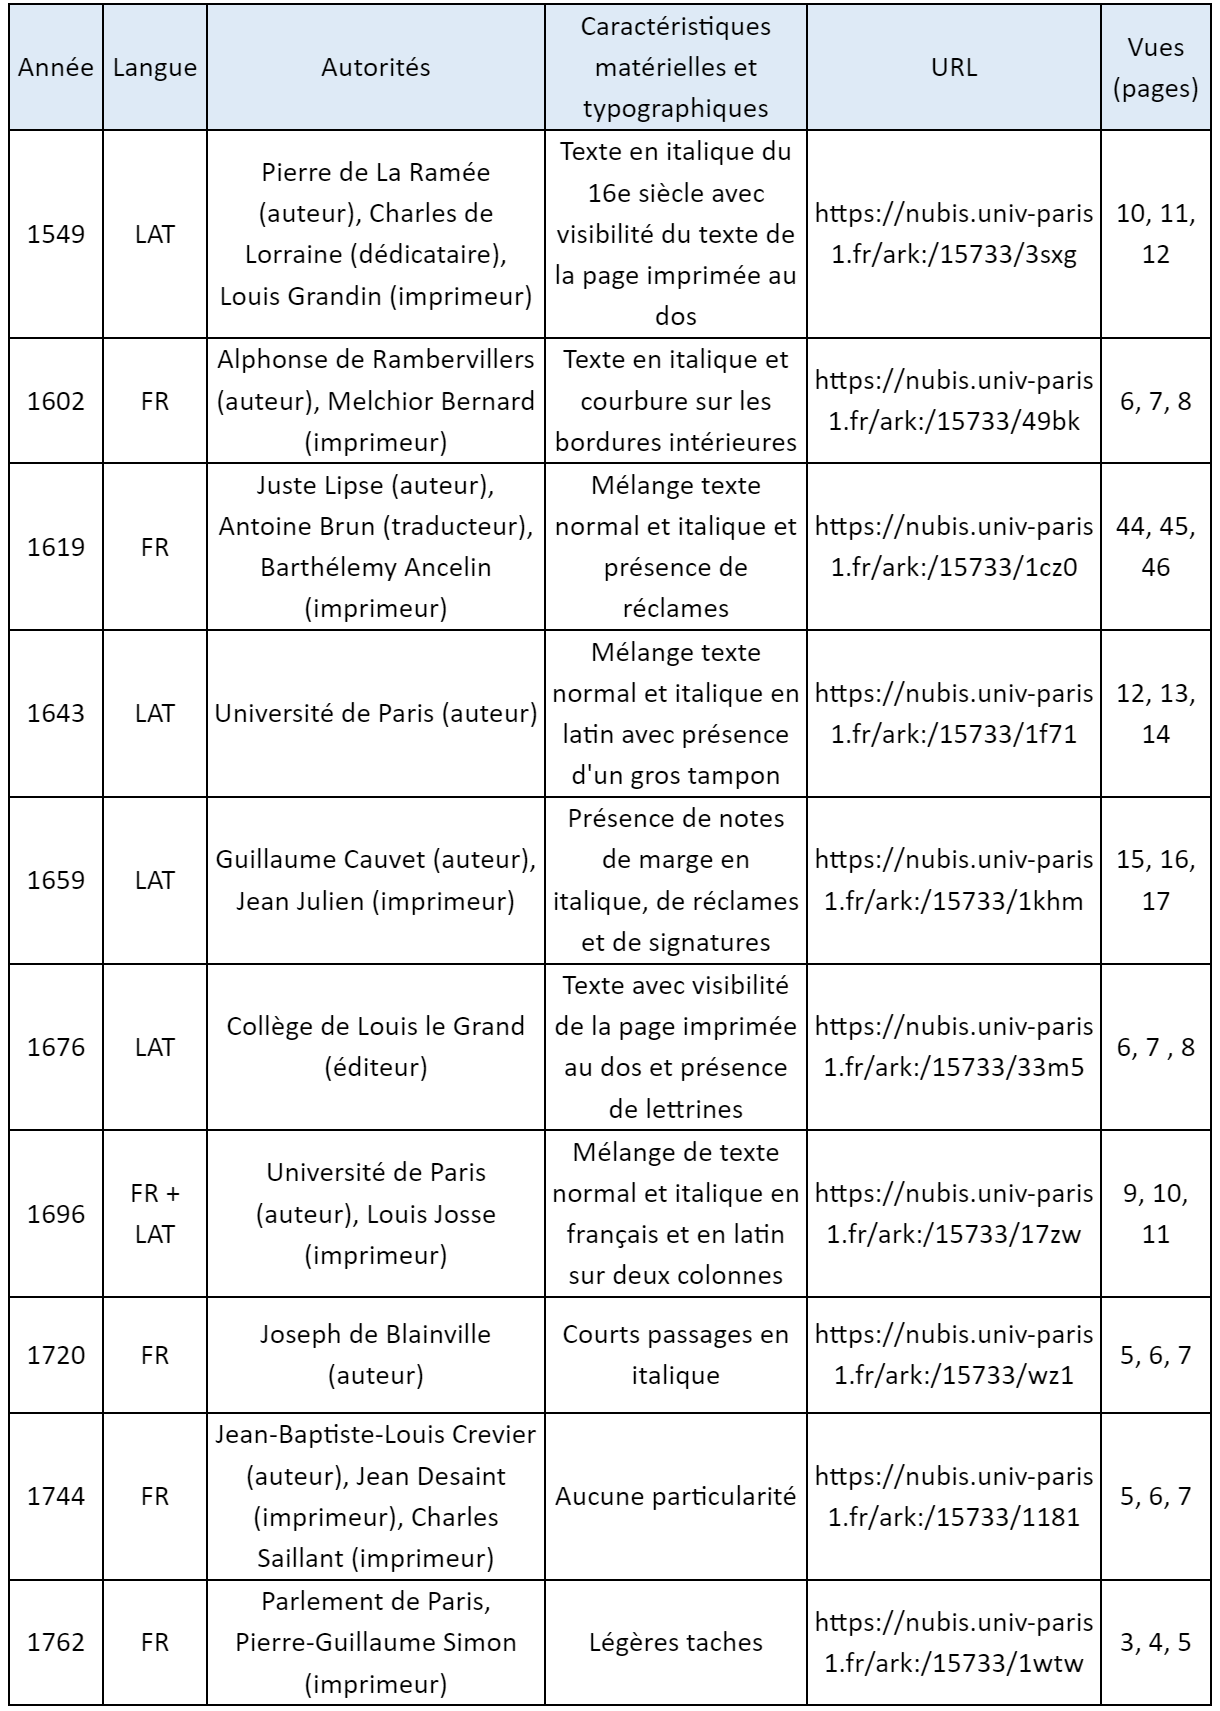
\includegraphics[width=6in,height=7.8in]{vertopal_157ae480aa4a4b07be198b586a812241/media/image21.png}
\end{table}

\begin{table} [H]
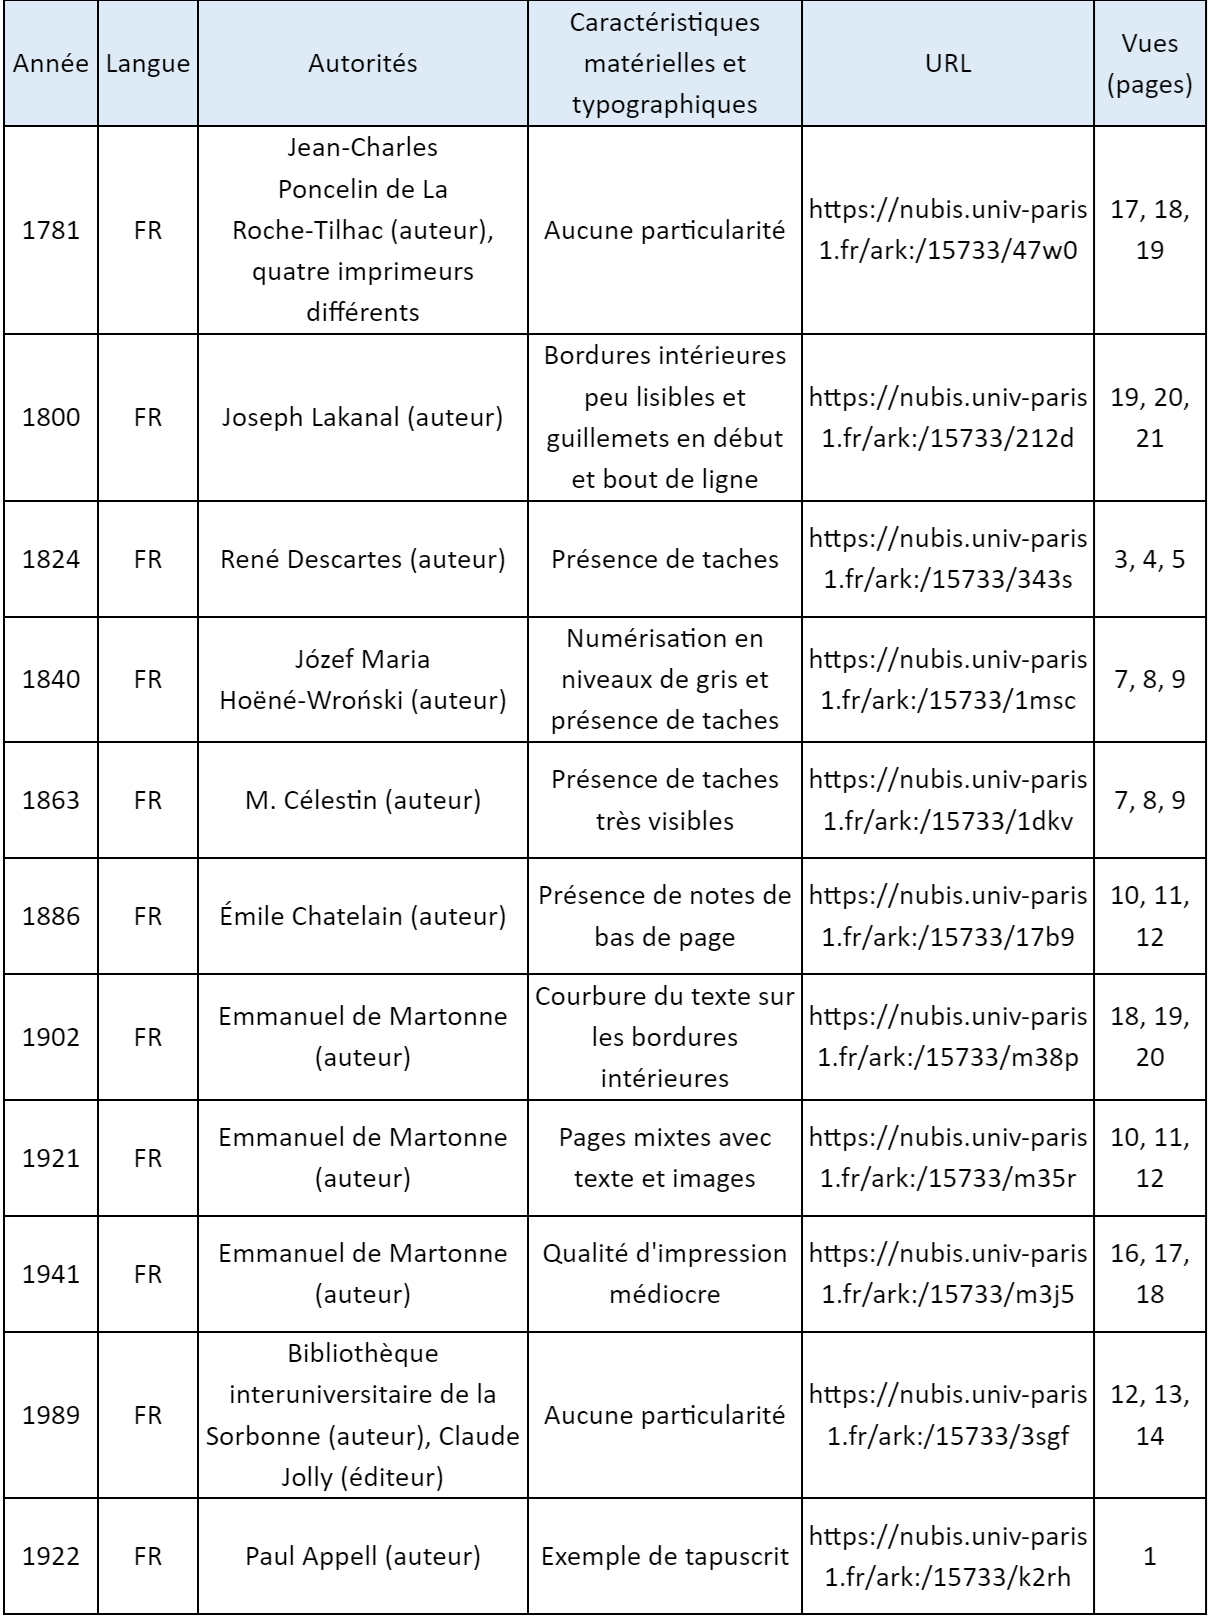
\includegraphics[width=6in,height=8.11944in]{vertopal_157ae480aa4a4b07be198b586a812241/media/image22.png}	
\caption{Caractéristiques du corpus établi}
\end{table}


\begin{table} [H]
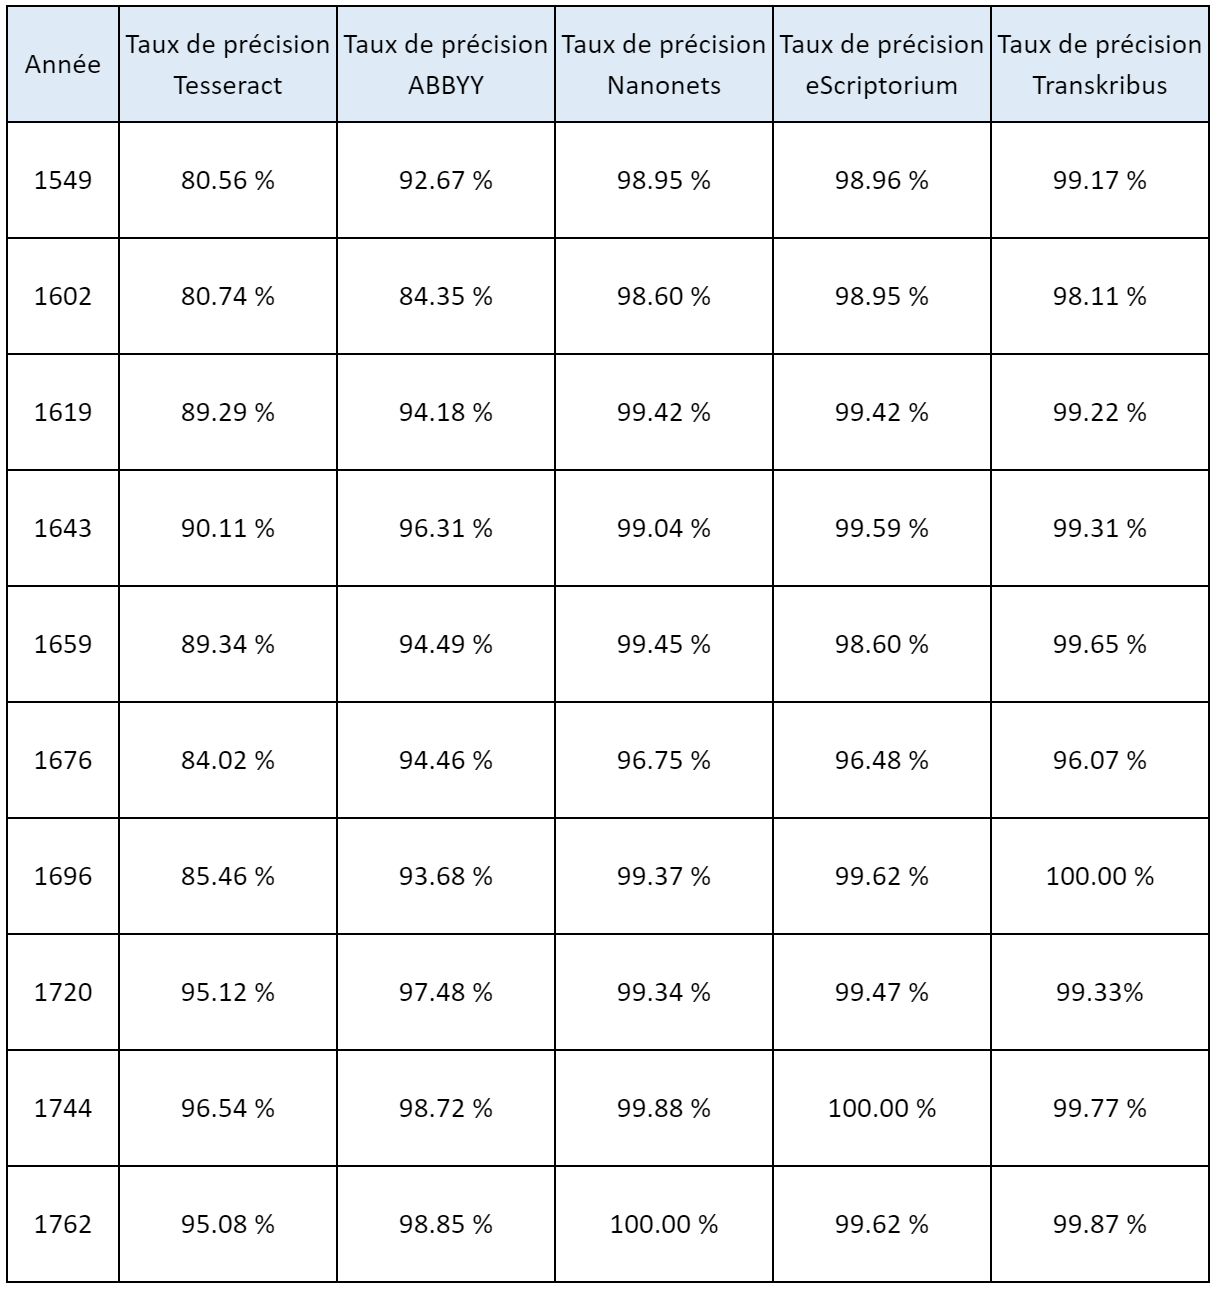
\includegraphics[width=6in,height=6.63889in]{vertopal_157ae480aa4a4b07be198b586a812241/media/image23.png}
\end{table}

\begin{table} [H]
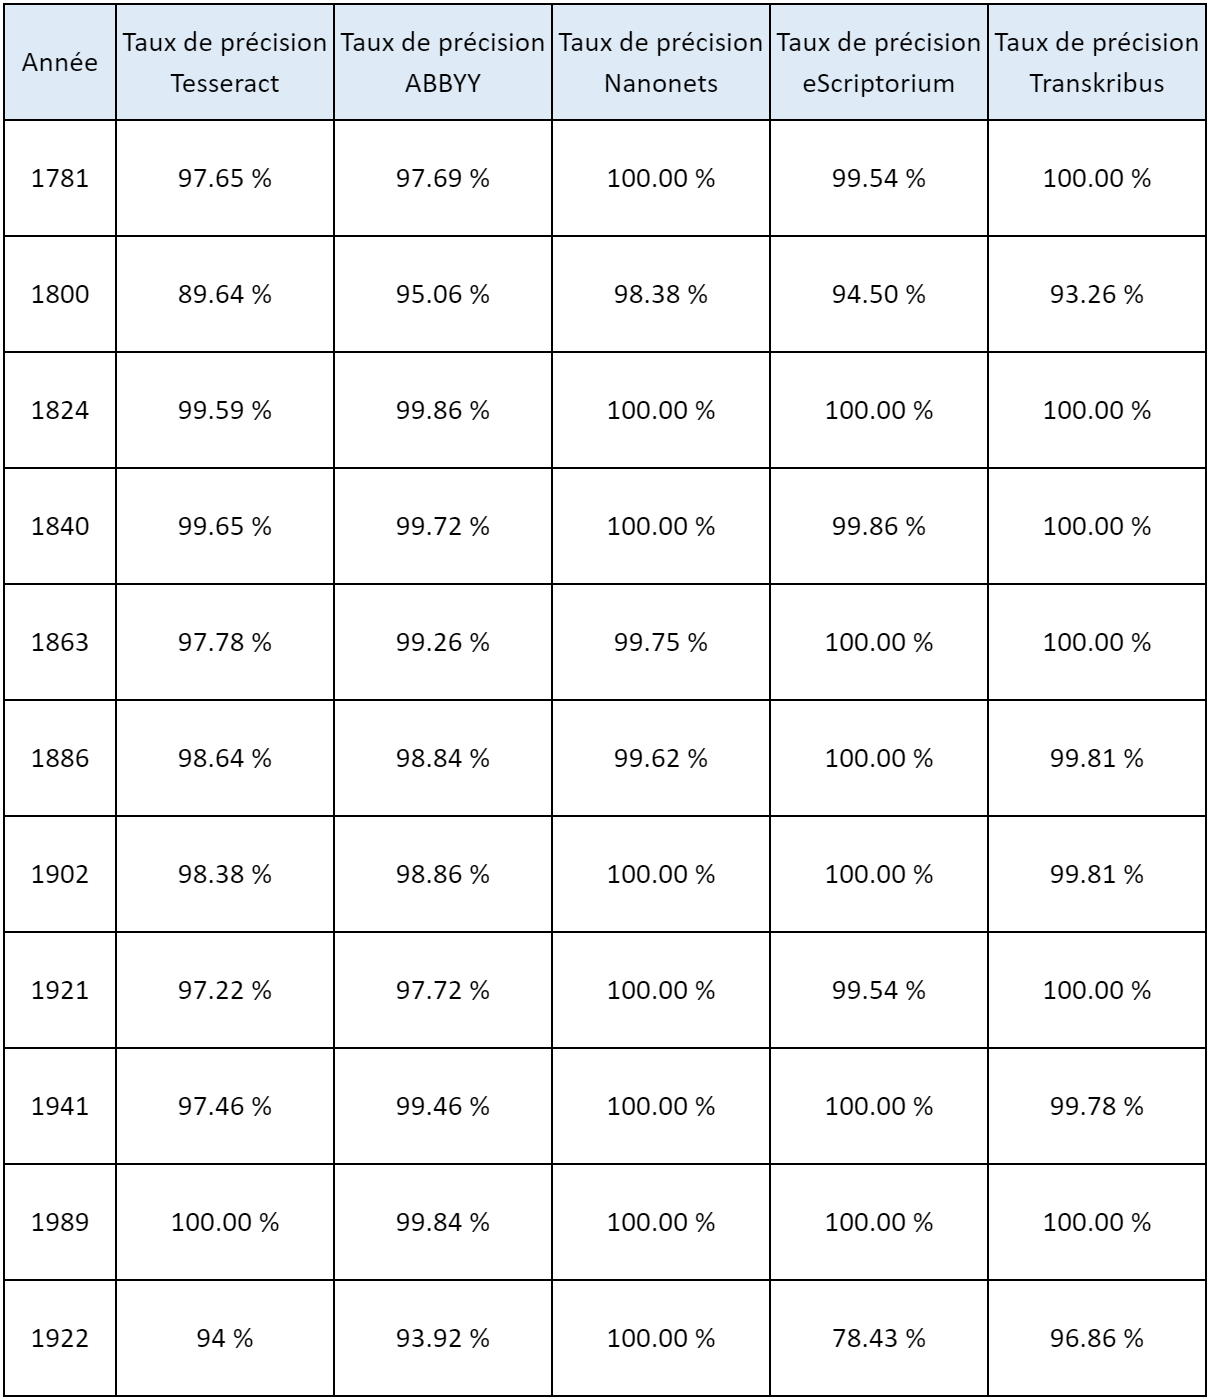
\includegraphics[width=6in,height=7.25in]{vertopal_157ae480aa4a4b07be198b586a812241/media/image24.png}
\caption{Taux de précision au mot des logiciels testés}
\end{table}

\newpage{\pagestyle{empty}\cleardoublepage}

%%%%%%%%%%%%%%%%%%

\backmatter % glossaire, index, table des figures, table des matières.. (la bibliographie a déjà été appelée)

%\printindex
%\printglossaries[title=Glossaire]
\listoftables
\listoffigures
\tableofcontents
\end{document}
